% Created by tikzDevice version 0.7.0 on 2014-06-29 19:48:01
% !TEX encoding = UTF-8 Unicode
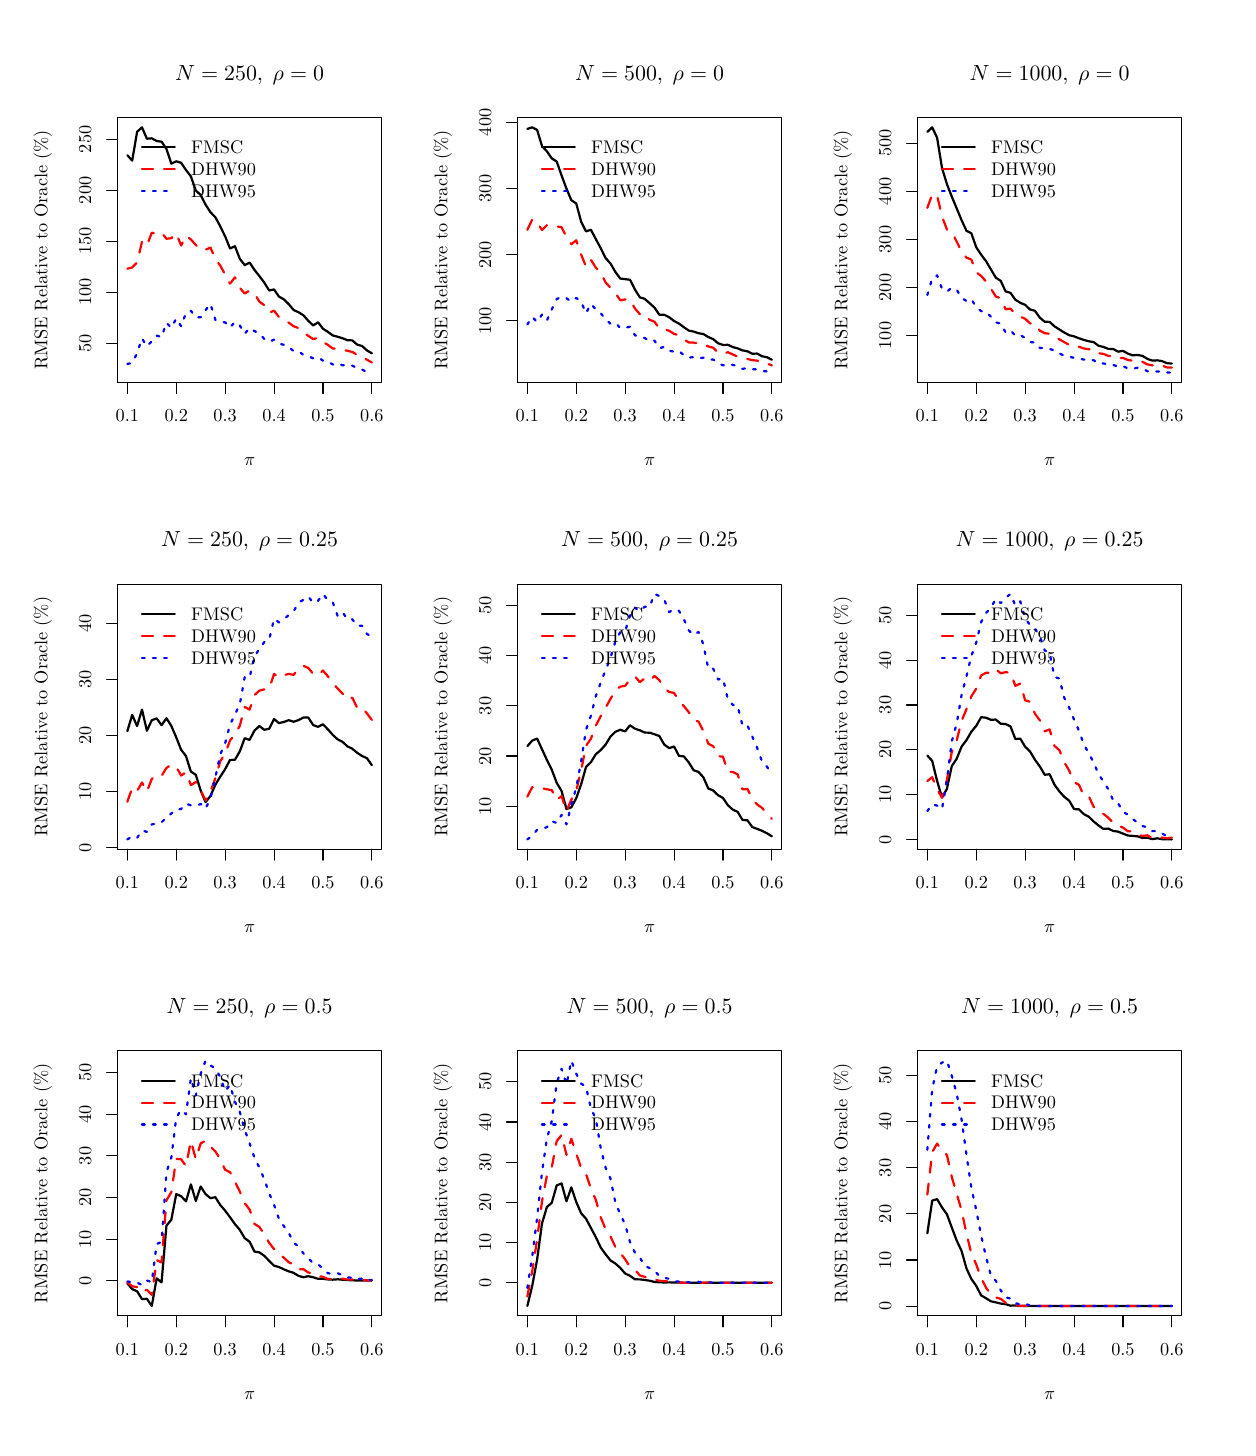
\begin{tikzpicture}[x=1pt,y=1pt]
\definecolor[named]{fillColor}{rgb}{1.00,1.00,1.00}
\path[use as bounding box,fill=fillColor,fill opacity=0.00] (0,0) rectangle (433.62,505.89);
\begin{scope}
\path[clip] ( 32.47,377.65) rectangle (127.91,473.42);
\definecolor[named]{drawColor}{rgb}{0.00,0.00,0.00}

\path[draw=drawColor,line width= 0.8pt,line join=round,line cap=round] ( 36.01,459.81) --
	( 37.77,457.84) --
	( 39.54,468.27) --
	( 41.31,469.87) --
	( 43.08,465.76) --
	( 44.84,465.90) --
	( 46.61,464.93) --
	( 48.38,464.68) --
	( 50.15,462.02) --
	( 51.91,456.74) --
	( 53.68,457.60) --
	( 55.45,457.07) --
	( 57.21,454.43) --
	( 58.98,452.15) --
	( 60.75,447.04) --
	( 62.52,445.43) --
	( 64.28,441.95) --
	( 66.05,439.20) --
	( 67.82,437.37) --
	( 69.59,434.08) --
	( 71.35,430.48) --
	( 73.12,426.10) --
	( 74.89,426.92) --
	( 76.66,422.36) --
	( 78.42,420.08) --
	( 80.19,421.00) --
	( 81.96,418.34) --
	( 83.72,416.13) --
	( 85.49,413.77) --
	( 87.26,410.92) --
	( 89.03,411.30) --
	( 90.79,408.72) --
	( 92.56,407.73) --
	( 94.33,405.97) --
	( 96.10,403.84) --
	( 97.86,403.07) --
	( 99.63,401.96) --
	(101.40,399.96) --
	(103.17,398.29) --
	(104.93,399.43) --
	(106.70,397.10) --
	(108.47,395.96) --
	(110.23,394.68) --
	(112.00,394.20) --
	(113.77,393.65) --
	(115.54,392.96) --
	(117.30,392.88) --
	(119.07,391.35) --
	(120.84,390.85) --
	(122.61,389.25) --
	(124.37,388.22);
\end{scope}
\begin{scope}
\path[clip] (  0.00,  0.00) rectangle (433.62,505.89);
\definecolor[named]{drawColor}{rgb}{0.00,0.00,0.00}

\path[draw=drawColor,line width= 0.4pt,line join=round,line cap=round] ( 36.01,377.65) -- (124.37,377.65);

\path[draw=drawColor,line width= 0.4pt,line join=round,line cap=round] ( 36.01,377.65) -- ( 36.01,373.69);

\path[draw=drawColor,line width= 0.4pt,line join=round,line cap=round] ( 53.68,377.65) -- ( 53.68,373.69);

\path[draw=drawColor,line width= 0.4pt,line join=round,line cap=round] ( 71.35,377.65) -- ( 71.35,373.69);

\path[draw=drawColor,line width= 0.4pt,line join=round,line cap=round] ( 89.03,377.65) -- ( 89.03,373.69);

\path[draw=drawColor,line width= 0.4pt,line join=round,line cap=round] (106.70,377.65) -- (106.70,373.69);

\path[draw=drawColor,line width= 0.4pt,line join=round,line cap=round] (124.37,377.65) -- (124.37,373.69);

\node[text=drawColor,anchor=base,inner sep=0pt, outer sep=0pt, scale=  0.66] at ( 36.01,363.40) {0.1};

\node[text=drawColor,anchor=base,inner sep=0pt, outer sep=0pt, scale=  0.66] at ( 53.68,363.40) {0.2};

\node[text=drawColor,anchor=base,inner sep=0pt, outer sep=0pt, scale=  0.66] at ( 71.35,363.40) {0.3};

\node[text=drawColor,anchor=base,inner sep=0pt, outer sep=0pt, scale=  0.66] at ( 89.03,363.40) {0.4};

\node[text=drawColor,anchor=base,inner sep=0pt, outer sep=0pt, scale=  0.66] at (106.70,363.40) {0.5};

\node[text=drawColor,anchor=base,inner sep=0pt, outer sep=0pt, scale=  0.66] at (124.37,363.40) {0.6};

\path[draw=drawColor,line width= 0.4pt,line join=round,line cap=round] ( 32.47,391.87) -- ( 32.47,465.53);

\path[draw=drawColor,line width= 0.4pt,line join=round,line cap=round] ( 32.47,391.87) -- ( 28.51,391.87);

\path[draw=drawColor,line width= 0.4pt,line join=round,line cap=round] ( 32.47,410.28) -- ( 28.51,410.28);

\path[draw=drawColor,line width= 0.4pt,line join=round,line cap=round] ( 32.47,428.70) -- ( 28.51,428.70);

\path[draw=drawColor,line width= 0.4pt,line join=round,line cap=round] ( 32.47,447.12) -- ( 28.51,447.12);

\path[draw=drawColor,line width= 0.4pt,line join=round,line cap=round] ( 32.47,465.53) -- ( 28.51,465.53);

\node[text=drawColor,rotate= 90.00,anchor=base,inner sep=0pt, outer sep=0pt, scale=  0.66] at ( 22.97,391.87) {50};

\node[text=drawColor,rotate= 90.00,anchor=base,inner sep=0pt, outer sep=0pt, scale=  0.66] at ( 22.97,410.28) {100};

\node[text=drawColor,rotate= 90.00,anchor=base,inner sep=0pt, outer sep=0pt, scale=  0.66] at ( 22.97,428.70) {150};

\node[text=drawColor,rotate= 90.00,anchor=base,inner sep=0pt, outer sep=0pt, scale=  0.66] at ( 22.97,447.12) {200};

\node[text=drawColor,rotate= 90.00,anchor=base,inner sep=0pt, outer sep=0pt, scale=  0.66] at ( 22.97,465.53) {250};

\path[draw=drawColor,line width= 0.4pt,line join=round,line cap=round] ( 32.47,377.65) --
	(127.91,377.65) --
	(127.91,473.42) --
	( 32.47,473.42) --
	( 32.47,377.65);
\end{scope}
\begin{scope}
\path[clip] (  0.00,337.26) rectangle (144.54,505.89);
\definecolor[named]{drawColor}{rgb}{0.00,0.00,0.00}

\node[text=drawColor,anchor=base,inner sep=0pt, outer sep=0pt, scale=  0.79] at ( 80.19,486.92) {\bfseries $N=250, \;\rho=0$};

\node[text=drawColor,anchor=base,inner sep=0pt, outer sep=0pt, scale=  0.66] at ( 80.19,347.56) {$\pi$};

\node[text=drawColor,rotate= 90.00,anchor=base,inner sep=0pt, outer sep=0pt, scale=  0.66] at (  7.13,425.53) {RMSE Relative to Oracle (\%)};
\end{scope}
\begin{scope}
\path[clip] ( 32.47,377.65) rectangle (127.91,473.42);
\definecolor[named]{drawColor}{rgb}{1.00,0.00,0.00}

\path[draw=drawColor,line width= 0.8pt,dash pattern=on 4pt off 4pt ,line join=round,line cap=round] ( 36.01,418.78) --
	( 37.77,419.24) --
	( 39.54,421.11) --
	( 41.31,428.52) --
	( 43.08,427.12) --
	( 44.84,431.79) --
	( 46.61,431.48) --
	( 48.38,431.83) --
	( 50.15,429.60) --
	( 51.91,429.82) --
	( 53.68,431.60) --
	( 55.45,427.16) --
	( 57.21,430.67) --
	( 58.98,429.37) --
	( 60.75,427.36) --
	( 62.52,425.68) --
	( 64.28,425.64) --
	( 66.05,426.43) --
	( 67.82,422.28) --
	( 69.59,419.93) --
	( 71.35,416.66) --
	( 73.12,413.40) --
	( 74.89,415.69) --
	( 76.66,411.85) --
	( 78.42,409.83) --
	( 80.19,410.86) --
	( 81.96,409.80) --
	( 83.72,406.88) --
	( 85.49,405.61) --
	( 87.26,402.91) --
	( 89.03,403.61) --
	( 90.79,401.34) --
	( 92.56,400.27) --
	( 94.33,399.27) --
	( 96.10,398.00) --
	( 97.86,397.33) --
	( 99.63,395.79) --
	(101.40,394.53) --
	(103.17,393.35) --
	(104.93,393.81) --
	(106.70,392.30) --
	(108.47,391.26) --
	(110.23,389.97) --
	(112.00,389.83) --
	(113.77,389.62) --
	(115.54,389.10) --
	(117.30,388.72) --
	(119.07,387.62) --
	(120.84,387.17) --
	(122.61,385.88) --
	(124.37,384.90);
\definecolor[named]{drawColor}{rgb}{0.00,0.00,1.00}

\path[draw=drawColor,line width= 0.8pt,dash pattern=on 1pt off 3pt ,line join=round,line cap=round] ( 36.01,384.39) --
	( 37.77,384.71) --
	( 39.54,388.29) --
	( 41.31,393.61) --
	( 43.08,390.72) --
	( 44.84,392.56) --
	( 46.61,394.61) --
	( 48.38,394.08) --
	( 50.15,399.26) --
	( 51.91,397.42) --
	( 53.68,400.79) --
	( 55.45,397.97) --
	( 57.21,402.86) --
	( 58.98,403.57) --
	( 60.75,401.21) --
	( 62.52,401.25) --
	( 64.28,403.82) --
	( 66.05,406.07) --
	( 67.82,400.30) --
	( 69.59,399.70) --
	( 71.35,399.39) --
	( 73.12,397.52) --
	( 74.89,399.60) --
	( 76.66,398.23) --
	( 78.42,395.26) --
	( 80.19,397.38) --
	( 81.96,396.25) --
	( 83.72,395.34) --
	( 85.49,393.42) --
	( 87.26,392.41) --
	( 89.03,393.15) --
	( 90.79,391.73) --
	( 92.56,391.29) --
	( 94.33,390.48) --
	( 96.10,389.02) --
	( 97.86,388.98) --
	( 99.63,387.63) --
	(101.40,387.14) --
	(103.17,386.43) --
	(104.93,386.79) --
	(106.70,385.57) --
	(108.47,385.34) --
	(110.23,384.18) --
	(112.00,384.54) --
	(113.77,383.89) --
	(115.54,384.07) --
	(117.30,383.75) --
	(119.07,382.89) --
	(120.84,382.32) --
	(122.61,381.44) --
	(124.37,381.20);
\definecolor[named]{drawColor}{rgb}{0.00,0.00,0.00}

\path[draw=drawColor,line width= 0.8pt,line join=round,line cap=round] ( 41.28,462.63) -- ( 53.16,462.63);
\definecolor[named]{drawColor}{rgb}{1.00,0.00,0.00}

\path[draw=drawColor,line width= 0.8pt,dash pattern=on 4pt off 4pt ,line join=round,line cap=round] ( 41.28,454.71) -- ( 53.16,454.71);
\definecolor[named]{drawColor}{rgb}{0.00,0.00,1.00}

\path[draw=drawColor,line width= 0.8pt,dash pattern=on 1pt off 3pt ,line join=round,line cap=round] ( 41.28,446.79) -- ( 53.16,446.79);
\definecolor[named]{drawColor}{rgb}{0.00,0.00,0.00}

\node[text=drawColor,anchor=base west,inner sep=0pt, outer sep=0pt, scale=  0.66] at ( 59.10,460.35) {FMSC};

\node[text=drawColor,anchor=base west,inner sep=0pt, outer sep=0pt, scale=  0.66] at ( 59.10,452.43) {DHW90};

\node[text=drawColor,anchor=base west,inner sep=0pt, outer sep=0pt, scale=  0.66] at ( 59.10,444.51) {DHW95};
\end{scope}
\begin{scope}
\path[clip] (177.01,377.65) rectangle (272.45,473.42);
\definecolor[named]{drawColor}{rgb}{0.00,0.00,0.00}

\path[draw=drawColor,line width= 0.8pt,line join=round,line cap=round] (180.55,469.31) --
	(182.31,469.87) --
	(184.08,468.96) --
	(185.85,463.11) --
	(187.62,461.19) --
	(189.38,458.64) --
	(191.15,457.54) --
	(192.92,452.49) --
	(194.69,447.73) --
	(196.45,443.54) --
	(198.22,442.36) --
	(199.99,435.81) --
	(201.75,432.27) --
	(203.52,432.86) --
	(205.29,429.50) --
	(207.06,426.23) --
	(208.82,422.66) --
	(210.59,420.66) --
	(212.36,417.63) --
	(214.13,415.23) --
	(215.89,415.02) --
	(217.66,414.78) --
	(219.43,411.25) --
	(221.20,408.45) --
	(222.96,407.89) --
	(224.73,406.33) --
	(226.50,404.74) --
	(228.26,402.13) --
	(230.03,402.15) --
	(231.80,401.25) --
	(233.57,399.89) --
	(235.33,398.97) --
	(237.10,397.66) --
	(238.87,396.43) --
	(240.64,396.07) --
	(242.40,395.47) --
	(244.17,395.18) --
	(245.94,394.10) --
	(247.71,393.33) --
	(249.47,391.85) --
	(251.24,391.25) --
	(253.01,391.28) --
	(254.77,390.48) --
	(256.54,389.99) --
	(258.31,389.27) --
	(260.08,388.94) --
	(261.84,388.07) --
	(263.61,388.12) --
	(265.38,387.15) --
	(267.15,386.79) --
	(268.91,385.90);
\end{scope}
\begin{scope}
\path[clip] (  0.00,  0.00) rectangle (433.62,505.89);
\definecolor[named]{drawColor}{rgb}{0.00,0.00,0.00}

\path[draw=drawColor,line width= 0.4pt,line join=round,line cap=round] (180.55,377.65) -- (268.91,377.65);

\path[draw=drawColor,line width= 0.4pt,line join=round,line cap=round] (180.55,377.65) -- (180.55,373.69);

\path[draw=drawColor,line width= 0.4pt,line join=round,line cap=round] (198.22,377.65) -- (198.22,373.69);

\path[draw=drawColor,line width= 0.4pt,line join=round,line cap=round] (215.89,377.65) -- (215.89,373.69);

\path[draw=drawColor,line width= 0.4pt,line join=round,line cap=round] (233.57,377.65) -- (233.57,373.69);

\path[draw=drawColor,line width= 0.4pt,line join=round,line cap=round] (251.24,377.65) -- (251.24,373.69);

\path[draw=drawColor,line width= 0.4pt,line join=round,line cap=round] (268.91,377.65) -- (268.91,373.69);

\node[text=drawColor,anchor=base,inner sep=0pt, outer sep=0pt, scale=  0.66] at (180.55,363.40) {0.1};

\node[text=drawColor,anchor=base,inner sep=0pt, outer sep=0pt, scale=  0.66] at (198.22,363.40) {0.2};

\node[text=drawColor,anchor=base,inner sep=0pt, outer sep=0pt, scale=  0.66] at (215.89,363.40) {0.3};

\node[text=drawColor,anchor=base,inner sep=0pt, outer sep=0pt, scale=  0.66] at (233.57,363.40) {0.4};

\node[text=drawColor,anchor=base,inner sep=0pt, outer sep=0pt, scale=  0.66] at (251.24,363.40) {0.5};

\node[text=drawColor,anchor=base,inner sep=0pt, outer sep=0pt, scale=  0.66] at (268.91,363.40) {0.6};

\path[draw=drawColor,line width= 0.4pt,line join=round,line cap=round] (177.01,400.02) -- (177.01,471.66);

\path[draw=drawColor,line width= 0.4pt,line join=round,line cap=round] (177.01,400.02) -- (173.05,400.02);

\path[draw=drawColor,line width= 0.4pt,line join=round,line cap=round] (177.01,423.90) -- (173.05,423.90);

\path[draw=drawColor,line width= 0.4pt,line join=round,line cap=round] (177.01,447.78) -- (173.05,447.78);

\path[draw=drawColor,line width= 0.4pt,line join=round,line cap=round] (177.01,471.66) -- (173.05,471.66);

\node[text=drawColor,rotate= 90.00,anchor=base,inner sep=0pt, outer sep=0pt, scale=  0.66] at (167.51,400.02) {100};

\node[text=drawColor,rotate= 90.00,anchor=base,inner sep=0pt, outer sep=0pt, scale=  0.66] at (167.51,423.90) {200};

\node[text=drawColor,rotate= 90.00,anchor=base,inner sep=0pt, outer sep=0pt, scale=  0.66] at (167.51,447.78) {300};

\node[text=drawColor,rotate= 90.00,anchor=base,inner sep=0pt, outer sep=0pt, scale=  0.66] at (167.51,471.66) {400};

\path[draw=drawColor,line width= 0.4pt,line join=round,line cap=round] (177.01,377.65) --
	(272.45,377.65) --
	(272.45,473.42) --
	(177.01,473.42) --
	(177.01,377.65);
\end{scope}
\begin{scope}
\path[clip] (144.54,337.26) rectangle (289.08,505.89);
\definecolor[named]{drawColor}{rgb}{0.00,0.00,0.00}

\node[text=drawColor,anchor=base,inner sep=0pt, outer sep=0pt, scale=  0.79] at (224.73,486.92) {\bfseries $N=500, \;\rho=0$};

\node[text=drawColor,anchor=base,inner sep=0pt, outer sep=0pt, scale=  0.66] at (224.73,347.56) {$\pi$};

\node[text=drawColor,rotate= 90.00,anchor=base,inner sep=0pt, outer sep=0pt, scale=  0.66] at (151.67,425.53) {RMSE Relative to Oracle (\%)};
\end{scope}
\begin{scope}
\path[clip] (177.01,377.65) rectangle (272.45,473.42);
\definecolor[named]{drawColor}{rgb}{1.00,0.00,0.00}

\path[draw=drawColor,line width= 0.8pt,dash pattern=on 4pt off 4pt ,line join=round,line cap=round] (180.55,432.81) --
	(182.31,436.56) --
	(184.08,435.62) --
	(185.85,432.76) --
	(187.62,434.50) --
	(189.38,434.37) --
	(191.15,434.06) --
	(192.92,433.78) --
	(194.69,430.27) --
	(196.45,427.64) --
	(198.22,429.05) --
	(199.99,423.90) --
	(201.75,419.55) --
	(203.52,422.01) --
	(205.29,419.15) --
	(207.06,417.43) --
	(208.82,413.83) --
	(210.59,411.94) --
	(212.36,410.03) --
	(214.13,407.38) --
	(215.89,407.68) --
	(217.66,407.53) --
	(219.43,404.40) --
	(221.20,402.38) --
	(222.96,402.32) --
	(224.73,400.34) --
	(226.50,399.64) --
	(228.26,397.14) --
	(230.03,396.96) --
	(231.80,396.36) --
	(233.57,395.23) --
	(235.33,394.73) --
	(237.10,393.32) --
	(238.87,392.12) --
	(240.64,392.08) --
	(242.40,391.71) --
	(244.17,391.56) --
	(245.94,390.69) --
	(247.71,390.22) --
	(249.47,388.51) --
	(251.24,388.06) --
	(253.01,388.60) --
	(254.77,387.81) --
	(256.54,387.01) --
	(258.31,386.57) --
	(260.08,386.17) --
	(261.84,385.75) --
	(263.61,385.56) --
	(265.38,384.82) --
	(267.15,384.55) --
	(268.91,383.83);
\definecolor[named]{drawColor}{rgb}{0.00,0.00,1.00}

\path[draw=drawColor,line width= 0.8pt,dash pattern=on 1pt off 3pt ,line join=round,line cap=round] (180.55,398.66) --
	(182.31,401.35) --
	(184.08,399.55) --
	(185.85,402.20) --
	(187.62,400.06) --
	(189.38,404.10) --
	(191.15,407.82) --
	(192.92,408.61) --
	(194.69,408.10) --
	(196.45,406.91) --
	(198.22,408.23) --
	(199.99,406.88) --
	(201.75,402.69) --
	(203.52,406.05) --
	(205.29,404.07) --
	(207.06,402.74) --
	(208.82,400.49) --
	(210.59,398.92) --
	(212.36,399.28) --
	(214.13,397.32) --
	(215.89,397.43) --
	(217.66,397.83) --
	(219.43,394.75) --
	(221.20,394.09) --
	(222.96,393.75) --
	(224.73,392.54) --
	(226.50,392.80) --
	(228.26,390.03) --
	(230.03,390.57) --
	(231.80,389.14) --
	(233.57,388.83) --
	(235.33,389.05) --
	(237.10,387.54) --
	(238.87,386.64) --
	(240.64,386.85) --
	(242.40,386.37) --
	(244.17,386.66) --
	(245.94,385.96) --
	(247.71,385.94) --
	(249.47,384.71) --
	(251.24,383.87) --
	(253.01,384.33) --
	(254.77,384.03) --
	(256.54,383.58) --
	(258.31,382.59) --
	(260.08,382.91) --
	(261.84,382.51) --
	(263.61,382.43) --
	(265.38,381.83) --
	(267.15,381.67) --
	(268.91,381.20);
\definecolor[named]{drawColor}{rgb}{0.00,0.00,0.00}

\path[draw=drawColor,line width= 0.8pt,line join=round,line cap=round] (185.82,462.63) -- (197.70,462.63);
\definecolor[named]{drawColor}{rgb}{1.00,0.00,0.00}

\path[draw=drawColor,line width= 0.8pt,dash pattern=on 4pt off 4pt ,line join=round,line cap=round] (185.82,454.71) -- (197.70,454.71);
\definecolor[named]{drawColor}{rgb}{0.00,0.00,1.00}

\path[draw=drawColor,line width= 0.8pt,dash pattern=on 1pt off 3pt ,line join=round,line cap=round] (185.82,446.79) -- (197.70,446.79);
\definecolor[named]{drawColor}{rgb}{0.00,0.00,0.00}

\node[text=drawColor,anchor=base west,inner sep=0pt, outer sep=0pt, scale=  0.66] at (203.64,460.35) {FMSC};

\node[text=drawColor,anchor=base west,inner sep=0pt, outer sep=0pt, scale=  0.66] at (203.64,452.43) {DHW90};

\node[text=drawColor,anchor=base west,inner sep=0pt, outer sep=0pt, scale=  0.66] at (203.64,444.51) {DHW95};
\end{scope}
\begin{scope}
\path[clip] (321.55,377.65) rectangle (416.99,473.42);
\definecolor[named]{drawColor}{rgb}{0.00,0.00,0.00}

\path[draw=drawColor,line width= 0.8pt,line join=round,line cap=round] (325.09,468.21) --
	(326.85,469.87) --
	(328.62,466.10) --
	(330.39,455.18) --
	(332.16,449.38) --
	(333.92,444.86) --
	(335.69,440.59) --
	(337.46,436.32) --
	(339.23,432.49) --
	(340.99,431.58) --
	(342.76,426.55) --
	(344.53,423.85) --
	(346.29,421.55) --
	(348.06,418.53) --
	(349.83,415.56) --
	(351.60,414.41) --
	(353.36,410.59) --
	(355.13,410.06) --
	(356.90,407.56) --
	(358.67,406.47) --
	(360.43,405.73) --
	(362.20,404.04) --
	(363.97,403.59) --
	(365.74,401.09) --
	(367.50,399.61) --
	(369.27,399.57) --
	(371.04,397.95) --
	(372.80,396.83) --
	(374.57,395.72) --
	(376.34,394.76) --
	(378.11,394.34) --
	(379.87,393.65) --
	(381.64,393.07) --
	(383.41,392.56) --
	(385.18,392.27) --
	(386.94,390.95) --
	(388.71,390.52) --
	(390.48,389.82) --
	(392.25,389.79) --
	(394.01,388.81) --
	(395.78,389.10) --
	(397.55,388.11) --
	(399.31,387.47) --
	(401.08,387.64) --
	(402.85,387.27) --
	(404.62,386.20) --
	(406.38,385.60) --
	(408.15,385.68) --
	(409.92,385.39) --
	(411.69,384.63) --
	(413.45,384.53);
\end{scope}
\begin{scope}
\path[clip] (  0.00,  0.00) rectangle (433.62,505.89);
\definecolor[named]{drawColor}{rgb}{0.00,0.00,0.00}

\path[draw=drawColor,line width= 0.4pt,line join=round,line cap=round] (325.09,377.65) -- (413.45,377.65);

\path[draw=drawColor,line width= 0.4pt,line join=round,line cap=round] (325.09,377.65) -- (325.09,373.69);

\path[draw=drawColor,line width= 0.4pt,line join=round,line cap=round] (342.76,377.65) -- (342.76,373.69);

\path[draw=drawColor,line width= 0.4pt,line join=round,line cap=round] (360.43,377.65) -- (360.43,373.69);

\path[draw=drawColor,line width= 0.4pt,line join=round,line cap=round] (378.11,377.65) -- (378.11,373.69);

\path[draw=drawColor,line width= 0.4pt,line join=round,line cap=round] (395.78,377.65) -- (395.78,373.69);

\path[draw=drawColor,line width= 0.4pt,line join=round,line cap=round] (413.45,377.65) -- (413.45,373.69);

\node[text=drawColor,anchor=base,inner sep=0pt, outer sep=0pt, scale=  0.66] at (325.09,363.40) {0.1};

\node[text=drawColor,anchor=base,inner sep=0pt, outer sep=0pt, scale=  0.66] at (342.76,363.40) {0.2};

\node[text=drawColor,anchor=base,inner sep=0pt, outer sep=0pt, scale=  0.66] at (360.43,363.40) {0.3};

\node[text=drawColor,anchor=base,inner sep=0pt, outer sep=0pt, scale=  0.66] at (378.11,363.40) {0.4};

\node[text=drawColor,anchor=base,inner sep=0pt, outer sep=0pt, scale=  0.66] at (395.78,363.40) {0.5};

\node[text=drawColor,anchor=base,inner sep=0pt, outer sep=0pt, scale=  0.66] at (413.45,363.40) {0.6};

\path[draw=drawColor,line width= 0.4pt,line join=round,line cap=round] (321.55,394.64) -- (321.55,464.11);

\path[draw=drawColor,line width= 0.4pt,line join=round,line cap=round] (321.55,394.64) -- (317.59,394.64);

\path[draw=drawColor,line width= 0.4pt,line join=round,line cap=round] (321.55,412.01) -- (317.59,412.01);

\path[draw=drawColor,line width= 0.4pt,line join=round,line cap=round] (321.55,429.37) -- (317.59,429.37);

\path[draw=drawColor,line width= 0.4pt,line join=round,line cap=round] (321.55,446.74) -- (317.59,446.74);

\path[draw=drawColor,line width= 0.4pt,line join=round,line cap=round] (321.55,464.11) -- (317.59,464.11);

\node[text=drawColor,rotate= 90.00,anchor=base,inner sep=0pt, outer sep=0pt, scale=  0.66] at (312.05,394.64) {100};

\node[text=drawColor,rotate= 90.00,anchor=base,inner sep=0pt, outer sep=0pt, scale=  0.66] at (312.05,412.01) {200};

\node[text=drawColor,rotate= 90.00,anchor=base,inner sep=0pt, outer sep=0pt, scale=  0.66] at (312.05,429.37) {300};

\node[text=drawColor,rotate= 90.00,anchor=base,inner sep=0pt, outer sep=0pt, scale=  0.66] at (312.05,446.74) {400};

\node[text=drawColor,rotate= 90.00,anchor=base,inner sep=0pt, outer sep=0pt, scale=  0.66] at (312.05,464.11) {500};

\path[draw=drawColor,line width= 0.4pt,line join=round,line cap=round] (321.55,377.65) --
	(416.99,377.65) --
	(416.99,473.42) --
	(321.55,473.42) --
	(321.55,377.65);
\end{scope}
\begin{scope}
\path[clip] (289.08,337.26) rectangle (433.62,505.89);
\definecolor[named]{drawColor}{rgb}{0.00,0.00,0.00}

\node[text=drawColor,anchor=base,inner sep=0pt, outer sep=0pt, scale=  0.79] at (369.27,486.92) {\bfseries $N=1000, \;\rho=0$};

\node[text=drawColor,anchor=base,inner sep=0pt, outer sep=0pt, scale=  0.66] at (369.27,347.56) {$\pi$};

\node[text=drawColor,rotate= 90.00,anchor=base,inner sep=0pt, outer sep=0pt, scale=  0.66] at (296.21,425.53) {RMSE Relative to Oracle (\%)};
\end{scope}
\begin{scope}
\path[clip] (321.55,377.65) rectangle (416.99,473.42);
\definecolor[named]{drawColor}{rgb}{1.00,0.00,0.00}

\path[draw=drawColor,line width= 0.8pt,dash pattern=on 4pt off 4pt ,line join=round,line cap=round] (325.09,440.75) --
	(326.85,445.68) --
	(328.62,445.25) --
	(330.39,437.66) --
	(332.16,432.98) --
	(333.92,432.07) --
	(335.69,428.59) --
	(337.46,425.01) --
	(339.23,422.75) --
	(340.99,422.09) --
	(342.76,417.46) --
	(344.53,416.19) --
	(346.29,414.16) --
	(348.06,411.56) --
	(349.83,408.74) --
	(351.60,408.09) --
	(353.36,404.14) --
	(355.13,404.37) --
	(356.90,402.38) --
	(358.67,401.47) --
	(360.43,400.69) --
	(362.20,399.04) --
	(363.97,398.80) --
	(365.74,396.41) --
	(367.50,395.47) --
	(369.27,395.27) --
	(371.04,394.09) --
	(372.80,393.26) --
	(374.57,392.24) --
	(376.34,391.29) --
	(378.11,391.14) --
	(379.87,390.58) --
	(381.64,389.95) --
	(383.41,389.69) --
	(385.18,389.44) --
	(386.94,388.26) --
	(388.71,388.00) --
	(390.48,387.29) --
	(392.25,387.25) --
	(394.01,386.47) --
	(395.78,386.55) --
	(397.55,385.81) --
	(399.31,385.52) --
	(401.08,385.51) --
	(402.85,385.12) --
	(404.62,384.20) --
	(406.38,383.88) --
	(408.15,383.96) --
	(409.92,383.78) --
	(411.69,383.12) --
	(413.45,383.04);
\definecolor[named]{drawColor}{rgb}{0.00,0.00,1.00}

\path[draw=drawColor,line width= 0.8pt,dash pattern=on 1pt off 3pt ,line join=round,line cap=round] (325.09,409.28) --
	(326.85,415.34) --
	(328.62,416.34) --
	(330.39,411.58) --
	(332.16,410.52) --
	(333.92,411.90) --
	(335.69,411.22) --
	(337.46,408.25) --
	(339.23,407.12) --
	(340.99,407.80) --
	(342.76,404.90) --
	(344.53,403.47) --
	(346.29,403.25) --
	(348.06,401.43) --
	(349.83,399.41) --
	(351.60,398.94) --
	(353.36,395.80) --
	(355.13,396.50) --
	(356.90,394.62) --
	(358.67,394.81) --
	(360.43,393.74) --
	(362.20,392.28) --
	(363.97,392.12) --
	(365.74,390.19) --
	(367.50,390.03) --
	(369.27,389.78) --
	(371.04,389.25) --
	(372.80,388.14) --
	(374.57,387.37) --
	(376.34,386.97) --
	(378.11,386.58) --
	(379.87,386.31) --
	(381.64,385.96) --
	(383.41,385.70) --
	(385.18,385.73) --
	(386.94,384.50) --
	(388.71,384.58) --
	(390.48,384.13) --
	(392.25,384.02) --
	(394.01,383.40) --
	(395.78,383.52) --
	(397.55,382.82) --
	(399.31,382.69) --
	(401.08,382.98) --
	(402.85,382.70) --
	(404.62,381.74) --
	(406.38,381.80) --
	(408.15,381.62) --
	(409.92,381.77) --
	(411.69,381.29) --
	(413.45,381.20);
\definecolor[named]{drawColor}{rgb}{0.00,0.00,0.00}

\path[draw=drawColor,line width= 0.8pt,line join=round,line cap=round] (330.36,462.63) -- (342.24,462.63);
\definecolor[named]{drawColor}{rgb}{1.00,0.00,0.00}

\path[draw=drawColor,line width= 0.8pt,dash pattern=on 4pt off 4pt ,line join=round,line cap=round] (330.36,454.71) -- (342.24,454.71);
\definecolor[named]{drawColor}{rgb}{0.00,0.00,1.00}

\path[draw=drawColor,line width= 0.8pt,dash pattern=on 1pt off 3pt ,line join=round,line cap=round] (330.36,446.79) -- (342.24,446.79);
\definecolor[named]{drawColor}{rgb}{0.00,0.00,0.00}

\node[text=drawColor,anchor=base west,inner sep=0pt, outer sep=0pt, scale=  0.66] at (348.18,460.35) {FMSC};

\node[text=drawColor,anchor=base west,inner sep=0pt, outer sep=0pt, scale=  0.66] at (348.18,452.43) {DHW90};

\node[text=drawColor,anchor=base west,inner sep=0pt, outer sep=0pt, scale=  0.66] at (348.18,444.51) {DHW95};
\end{scope}
\begin{scope}
\path[clip] ( 32.47,209.02) rectangle (127.91,304.79);
\definecolor[named]{drawColor}{rgb}{0.00,0.00,0.00}

\path[draw=drawColor,line width= 0.8pt,line join=round,line cap=round] ( 36.01,251.68) --
	( 37.77,257.56) --
	( 39.54,253.52) --
	( 41.31,259.49) --
	( 43.08,251.82) --
	( 44.84,255.64) --
	( 46.61,256.30) --
	( 48.38,253.83) --
	( 50.15,256.36) --
	( 51.91,253.56) --
	( 53.68,249.45) --
	( 55.45,244.96) --
	( 57.21,242.65) --
	( 58.98,237.06) --
	( 60.75,235.92) --
	( 62.52,230.21) --
	( 64.28,226.02) --
	( 66.05,228.29) --
	( 67.82,232.32) --
	( 69.59,235.23) --
	( 71.35,237.95) --
	( 73.12,241.29) --
	( 74.89,241.33) --
	( 76.66,244.41) --
	( 78.42,249.13) --
	( 80.19,248.53) --
	( 81.96,251.91) --
	( 83.72,253.53) --
	( 85.49,252.18) --
	( 87.26,252.52) --
	( 89.03,256.06) --
	( 90.79,254.59) --
	( 92.56,255.01) --
	( 94.33,255.65) --
	( 96.10,255.08) --
	( 97.86,255.68) --
	( 99.63,256.61) --
	(101.40,256.61) --
	(103.17,253.88) --
	(104.93,253.24) --
	(106.70,254.15) --
	(108.47,252.35) --
	(110.23,250.35) --
	(112.00,248.74) --
	(113.77,247.81) --
	(115.54,246.19) --
	(117.30,245.33) --
	(119.07,243.85) --
	(120.84,242.71) --
	(122.61,241.89) --
	(124.37,239.37);
\end{scope}
\begin{scope}
\path[clip] (  0.00,  0.00) rectangle (433.62,505.89);
\definecolor[named]{drawColor}{rgb}{0.00,0.00,0.00}

\path[draw=drawColor,line width= 0.4pt,line join=round,line cap=round] ( 36.01,209.02) -- (124.37,209.02);

\path[draw=drawColor,line width= 0.4pt,line join=round,line cap=round] ( 36.01,209.02) -- ( 36.01,205.06);

\path[draw=drawColor,line width= 0.4pt,line join=round,line cap=round] ( 53.68,209.02) -- ( 53.68,205.06);

\path[draw=drawColor,line width= 0.4pt,line join=round,line cap=round] ( 71.35,209.02) -- ( 71.35,205.06);

\path[draw=drawColor,line width= 0.4pt,line join=round,line cap=round] ( 89.03,209.02) -- ( 89.03,205.06);

\path[draw=drawColor,line width= 0.4pt,line join=round,line cap=round] (106.70,209.02) -- (106.70,205.06);

\path[draw=drawColor,line width= 0.4pt,line join=round,line cap=round] (124.37,209.02) -- (124.37,205.06);

\node[text=drawColor,anchor=base,inner sep=0pt, outer sep=0pt, scale=  0.66] at ( 36.01,194.77) {0.1};

\node[text=drawColor,anchor=base,inner sep=0pt, outer sep=0pt, scale=  0.66] at ( 53.68,194.77) {0.2};

\node[text=drawColor,anchor=base,inner sep=0pt, outer sep=0pt, scale=  0.66] at ( 71.35,194.77) {0.3};

\node[text=drawColor,anchor=base,inner sep=0pt, outer sep=0pt, scale=  0.66] at ( 89.03,194.77) {0.4};

\node[text=drawColor,anchor=base,inner sep=0pt, outer sep=0pt, scale=  0.66] at (106.70,194.77) {0.5};

\node[text=drawColor,anchor=base,inner sep=0pt, outer sep=0pt, scale=  0.66] at (124.37,194.77) {0.6};

\path[draw=drawColor,line width= 0.4pt,line join=round,line cap=round] ( 32.47,209.63) -- ( 32.47,290.61);

\path[draw=drawColor,line width= 0.4pt,line join=round,line cap=round] ( 32.47,209.63) -- ( 28.51,209.63);

\path[draw=drawColor,line width= 0.4pt,line join=round,line cap=round] ( 32.47,229.87) -- ( 28.51,229.87);

\path[draw=drawColor,line width= 0.4pt,line join=round,line cap=round] ( 32.47,250.12) -- ( 28.51,250.12);

\path[draw=drawColor,line width= 0.4pt,line join=round,line cap=round] ( 32.47,270.37) -- ( 28.51,270.37);

\path[draw=drawColor,line width= 0.4pt,line join=round,line cap=round] ( 32.47,290.61) -- ( 28.51,290.61);

\node[text=drawColor,rotate= 90.00,anchor=base,inner sep=0pt, outer sep=0pt, scale=  0.66] at ( 22.97,209.63) {0};

\node[text=drawColor,rotate= 90.00,anchor=base,inner sep=0pt, outer sep=0pt, scale=  0.66] at ( 22.97,229.87) {10};

\node[text=drawColor,rotate= 90.00,anchor=base,inner sep=0pt, outer sep=0pt, scale=  0.66] at ( 22.97,250.12) {20};

\node[text=drawColor,rotate= 90.00,anchor=base,inner sep=0pt, outer sep=0pt, scale=  0.66] at ( 22.97,270.37) {30};

\node[text=drawColor,rotate= 90.00,anchor=base,inner sep=0pt, outer sep=0pt, scale=  0.66] at ( 22.97,290.61) {40};

\path[draw=drawColor,line width= 0.4pt,line join=round,line cap=round] ( 32.47,209.02) --
	(127.91,209.02) --
	(127.91,304.79) --
	( 32.47,304.79) --
	( 32.47,209.02);
\end{scope}
\begin{scope}
\path[clip] (  0.00,168.63) rectangle (144.54,337.26);
\definecolor[named]{drawColor}{rgb}{0.00,0.00,0.00}

\node[text=drawColor,anchor=base,inner sep=0pt, outer sep=0pt, scale=  0.79] at ( 80.19,318.29) {\bfseries $N=250, \;\rho=0.25$};

\node[text=drawColor,anchor=base,inner sep=0pt, outer sep=0pt, scale=  0.66] at ( 80.19,178.93) {$\pi$};

\node[text=drawColor,rotate= 90.00,anchor=base,inner sep=0pt, outer sep=0pt, scale=  0.66] at (  7.13,256.90) {RMSE Relative to Oracle (\%)};
\end{scope}
\begin{scope}
\path[clip] ( 32.47,209.02) rectangle (127.91,304.79);
\definecolor[named]{drawColor}{rgb}{1.00,0.00,0.00}

\path[draw=drawColor,line width= 0.8pt,dash pattern=on 4pt off 4pt ,line join=round,line cap=round] ( 36.01,226.15) --
	( 37.77,231.16) --
	( 39.54,230.02) --
	( 41.31,233.12) --
	( 43.08,229.85) --
	( 44.84,234.40) --
	( 46.61,235.68) --
	( 48.38,235.51) --
	( 50.15,238.39) --
	( 51.91,239.57) --
	( 53.68,238.74) --
	( 55.45,235.65) --
	( 57.21,236.80) --
	( 58.98,232.16) --
	( 60.75,233.30) --
	( 62.52,230.25) --
	( 64.28,226.67) --
	( 66.05,229.87) --
	( 67.82,234.67) --
	( 69.59,240.82) --
	( 71.35,243.54) --
	( 73.12,248.33) --
	( 74.89,250.49) --
	( 76.66,253.65) --
	( 78.42,260.43) --
	( 80.19,259.45) --
	( 81.96,264.70) --
	( 83.72,266.33) --
	( 85.49,266.78) --
	( 87.26,267.15) --
	( 89.03,272.31) --
	( 90.79,271.09) --
	( 92.56,271.88) --
	( 94.33,272.38) --
	( 96.10,272.02) --
	( 97.86,274.25) --
	( 99.63,275.28) --
	(101.40,274.52) --
	(103.17,272.35) --
	(104.93,271.96) --
	(106.70,273.59) --
	(108.47,271.53) --
	(110.23,269.00) --
	(112.00,267.09) --
	(113.77,265.26) --
	(115.54,263.17) --
	(117.30,263.76) --
	(119.07,260.11) --
	(120.84,260.21) --
	(122.61,258.05) --
	(124.37,255.74);
\definecolor[named]{drawColor}{rgb}{0.00,0.00,1.00}

\path[draw=drawColor,line width= 0.8pt,dash pattern=on 1pt off 3pt ,line join=round,line cap=round] ( 36.01,212.57) --
	( 37.77,213.59) --
	( 39.54,213.08) --
	( 41.31,215.80) --
	( 43.08,215.31) --
	( 44.84,217.98) --
	( 46.61,218.27) --
	( 48.38,218.76) --
	( 50.15,220.46) --
	( 51.91,221.93) --
	( 53.68,223.40) --
	( 55.45,223.54) --
	( 57.21,225.46) --
	( 58.98,224.87) --
	( 60.75,224.73) --
	( 62.52,225.36) --
	( 64.28,223.72) --
	( 66.05,227.39) --
	( 67.82,234.96) --
	( 69.59,243.30) --
	( 71.35,247.28) --
	( 73.12,254.08) --
	( 74.89,257.64) --
	( 76.66,261.45) --
	( 78.42,271.20) --
	( 80.19,271.04) --
	( 81.96,278.80) --
	( 83.72,281.31) --
	( 85.49,283.87) --
	( 87.26,284.69) --
	( 89.03,292.29) --
	( 90.79,290.98) --
	( 92.56,292.10) --
	( 94.33,293.65) --
	( 96.10,294.99) --
	( 97.86,298.13) --
	( 99.63,299.12) --
	(101.40,300.32) --
	(103.17,298.03) --
	(104.93,298.80) --
	(106.70,301.24) --
	(108.47,299.06) --
	(110.23,298.24) --
	(112.00,293.33) --
	(113.77,294.66) --
	(115.54,292.14) --
	(117.30,292.10) --
	(119.07,289.76) --
	(120.84,289.77) --
	(122.61,286.76) --
	(124.37,285.91);
\definecolor[named]{drawColor}{rgb}{0.00,0.00,0.00}

\path[draw=drawColor,line width= 0.8pt,line join=round,line cap=round] ( 41.28,294.00) -- ( 53.16,294.00);
\definecolor[named]{drawColor}{rgb}{1.00,0.00,0.00}

\path[draw=drawColor,line width= 0.8pt,dash pattern=on 4pt off 4pt ,line join=round,line cap=round] ( 41.28,286.08) -- ( 53.16,286.08);
\definecolor[named]{drawColor}{rgb}{0.00,0.00,1.00}

\path[draw=drawColor,line width= 0.8pt,dash pattern=on 1pt off 3pt ,line join=round,line cap=round] ( 41.28,278.16) -- ( 53.16,278.16);
\definecolor[named]{drawColor}{rgb}{0.00,0.00,0.00}

\node[text=drawColor,anchor=base west,inner sep=0pt, outer sep=0pt, scale=  0.66] at ( 59.10,291.72) {FMSC};

\node[text=drawColor,anchor=base west,inner sep=0pt, outer sep=0pt, scale=  0.66] at ( 59.10,283.80) {DHW90};

\node[text=drawColor,anchor=base west,inner sep=0pt, outer sep=0pt, scale=  0.66] at ( 59.10,275.88) {DHW95};
\end{scope}
\begin{scope}
\path[clip] (177.01,209.02) rectangle (272.45,304.79);
\definecolor[named]{drawColor}{rgb}{0.00,0.00,0.00}

\path[draw=drawColor,line width= 0.8pt,line join=round,line cap=round] (180.55,246.26) --
	(182.31,248.27) --
	(184.08,249.02) --
	(185.85,245.13) --
	(187.62,241.27) --
	(189.38,237.74) --
	(191.15,233.03) --
	(192.92,230.05) --
	(194.69,223.52) --
	(196.45,224.15) --
	(198.22,227.44) --
	(199.99,232.44) --
	(201.75,238.74) --
	(203.52,240.46) --
	(205.29,243.34) --
	(207.06,244.83) --
	(208.82,246.80) --
	(210.59,249.72) --
	(212.36,251.45) --
	(214.13,252.19) --
	(215.89,251.60) --
	(217.66,253.80) --
	(219.43,252.57) --
	(221.20,252.00) --
	(222.96,251.17) --
	(224.73,251.13) --
	(226.50,250.57) --
	(228.26,249.91) --
	(230.03,246.83) --
	(231.80,245.55) --
	(233.57,246.14) --
	(235.33,242.78) --
	(237.10,242.56) --
	(238.87,240.41) --
	(240.64,237.55) --
	(242.40,236.96) --
	(244.17,234.98) --
	(245.94,230.96) --
	(247.71,230.26) --
	(249.47,228.53) --
	(251.24,227.54) --
	(253.01,224.93) --
	(254.77,223.33) --
	(256.54,222.52) --
	(258.31,219.60) --
	(260.08,219.46) --
	(261.84,217.02) --
	(263.61,216.36) --
	(265.38,215.67) --
	(267.15,214.78) --
	(268.91,213.66);
\end{scope}
\begin{scope}
\path[clip] (  0.00,  0.00) rectangle (433.62,505.89);
\definecolor[named]{drawColor}{rgb}{0.00,0.00,0.00}

\path[draw=drawColor,line width= 0.4pt,line join=round,line cap=round] (180.55,209.02) -- (268.91,209.02);

\path[draw=drawColor,line width= 0.4pt,line join=round,line cap=round] (180.55,209.02) -- (180.55,205.06);

\path[draw=drawColor,line width= 0.4pt,line join=round,line cap=round] (198.22,209.02) -- (198.22,205.06);

\path[draw=drawColor,line width= 0.4pt,line join=round,line cap=round] (215.89,209.02) -- (215.89,205.06);

\path[draw=drawColor,line width= 0.4pt,line join=round,line cap=round] (233.57,209.02) -- (233.57,205.06);

\path[draw=drawColor,line width= 0.4pt,line join=round,line cap=round] (251.24,209.02) -- (251.24,205.06);

\path[draw=drawColor,line width= 0.4pt,line join=round,line cap=round] (268.91,209.02) -- (268.91,205.06);

\node[text=drawColor,anchor=base,inner sep=0pt, outer sep=0pt, scale=  0.66] at (180.55,194.77) {0.1};

\node[text=drawColor,anchor=base,inner sep=0pt, outer sep=0pt, scale=  0.66] at (198.22,194.77) {0.2};

\node[text=drawColor,anchor=base,inner sep=0pt, outer sep=0pt, scale=  0.66] at (215.89,194.77) {0.3};

\node[text=drawColor,anchor=base,inner sep=0pt, outer sep=0pt, scale=  0.66] at (233.57,194.77) {0.4};

\node[text=drawColor,anchor=base,inner sep=0pt, outer sep=0pt, scale=  0.66] at (251.24,194.77) {0.5};

\node[text=drawColor,anchor=base,inner sep=0pt, outer sep=0pt, scale=  0.66] at (268.91,194.77) {0.6};

\path[draw=drawColor,line width= 0.4pt,line join=round,line cap=round] (177.01,224.56) -- (177.01,297.07);

\path[draw=drawColor,line width= 0.4pt,line join=round,line cap=round] (177.01,224.56) -- (173.05,224.56);

\path[draw=drawColor,line width= 0.4pt,line join=round,line cap=round] (177.01,242.69) -- (173.05,242.69);

\path[draw=drawColor,line width= 0.4pt,line join=round,line cap=round] (177.01,260.81) -- (173.05,260.81);

\path[draw=drawColor,line width= 0.4pt,line join=round,line cap=round] (177.01,278.94) -- (173.05,278.94);

\path[draw=drawColor,line width= 0.4pt,line join=round,line cap=round] (177.01,297.07) -- (173.05,297.07);

\node[text=drawColor,rotate= 90.00,anchor=base,inner sep=0pt, outer sep=0pt, scale=  0.66] at (167.51,224.56) {10};

\node[text=drawColor,rotate= 90.00,anchor=base,inner sep=0pt, outer sep=0pt, scale=  0.66] at (167.51,242.69) {20};

\node[text=drawColor,rotate= 90.00,anchor=base,inner sep=0pt, outer sep=0pt, scale=  0.66] at (167.51,260.81) {30};

\node[text=drawColor,rotate= 90.00,anchor=base,inner sep=0pt, outer sep=0pt, scale=  0.66] at (167.51,278.94) {40};

\node[text=drawColor,rotate= 90.00,anchor=base,inner sep=0pt, outer sep=0pt, scale=  0.66] at (167.51,297.07) {50};

\path[draw=drawColor,line width= 0.4pt,line join=round,line cap=round] (177.01,209.02) --
	(272.45,209.02) --
	(272.45,304.79) --
	(177.01,304.79) --
	(177.01,209.02);
\end{scope}
\begin{scope}
\path[clip] (144.54,168.63) rectangle (289.08,337.26);
\definecolor[named]{drawColor}{rgb}{0.00,0.00,0.00}

\node[text=drawColor,anchor=base,inner sep=0pt, outer sep=0pt, scale=  0.79] at (224.73,318.29) {\bfseries $N=500, \;\rho=0.25$};

\node[text=drawColor,anchor=base,inner sep=0pt, outer sep=0pt, scale=  0.66] at (224.73,178.93) {$\pi$};

\node[text=drawColor,rotate= 90.00,anchor=base,inner sep=0pt, outer sep=0pt, scale=  0.66] at (151.67,256.90) {RMSE Relative to Oracle (\%)};
\end{scope}
\begin{scope}
\path[clip] (177.01,209.02) rectangle (272.45,304.79);
\definecolor[named]{drawColor}{rgb}{1.00,0.00,0.00}

\path[draw=drawColor,line width= 0.8pt,dash pattern=on 4pt off 4pt ,line join=round,line cap=round] (180.55,228.03) --
	(182.31,231.43) --
	(184.08,231.34) --
	(185.85,231.03) --
	(187.62,230.67) --
	(189.38,230.38) --
	(191.15,226.82) --
	(192.92,228.22) --
	(194.69,222.79) --
	(196.45,226.96) --
	(198.22,230.19) --
	(199.99,237.44) --
	(201.75,246.38) --
	(203.52,248.95) --
	(205.29,253.70) --
	(207.06,257.05) --
	(208.82,260.17) --
	(210.59,263.31) --
	(212.36,266.41) --
	(214.13,267.77) --
	(215.89,268.06) --
	(217.66,270.41) --
	(219.43,271.50) --
	(221.20,269.37) --
	(222.96,270.82) --
	(224.73,269.95) --
	(226.50,271.62) --
	(228.26,270.11) --
	(230.03,267.27) --
	(231.80,265.84) --
	(233.57,265.50) --
	(235.33,262.57) --
	(237.10,260.74) --
	(238.87,258.58) --
	(240.64,255.67) --
	(242.40,255.17) --
	(244.17,251.73) --
	(245.94,247.16) --
	(247.71,246.24) --
	(249.47,242.62) --
	(251.24,242.48) --
	(253.01,236.99) --
	(254.77,236.95) --
	(256.54,236.09) --
	(258.31,230.64) --
	(260.08,230.79) --
	(261.84,227.21) --
	(263.61,225.17) --
	(265.38,223.95) --
	(267.15,221.65) --
	(268.91,220.00);
\definecolor[named]{drawColor}{rgb}{0.00,0.00,1.00}

\path[draw=drawColor,line width= 0.8pt,dash pattern=on 1pt off 3pt ,line join=round,line cap=round] (180.55,212.57) --
	(182.31,213.83) --
	(184.08,216.05) --
	(185.85,216.37) --
	(187.62,217.01) --
	(189.38,219.13) --
	(191.15,218.50) --
	(192.92,221.42) --
	(194.69,217.98) --
	(196.45,225.07) --
	(198.22,231.23) --
	(199.99,240.76) --
	(201.75,252.20) --
	(203.52,257.26) --
	(205.29,264.35) --
	(207.06,269.24) --
	(208.82,273.75) --
	(210.59,278.15) --
	(212.36,284.09) --
	(214.13,287.48) --
	(215.89,287.74) --
	(217.66,293.48) --
	(219.43,296.28) --
	(221.20,295.12) --
	(222.96,296.61) --
	(224.73,296.58) --
	(226.50,301.24) --
	(228.26,300.52) --
	(230.03,299.18) --
	(231.80,294.71) --
	(233.57,295.75) --
	(235.33,295.16) --
	(237.10,292.18) --
	(238.87,288.12) --
	(240.64,286.44) --
	(242.40,287.53) --
	(244.17,282.98) --
	(245.94,274.23) --
	(247.71,274.22) --
	(249.47,270.36) --
	(251.24,270.74) --
	(253.01,263.19) --
	(254.77,261.20) --
	(256.54,260.82) --
	(258.31,253.66) --
	(260.08,253.78) --
	(261.84,249.70) --
	(263.61,245.59) --
	(265.38,240.64) --
	(267.15,238.87) --
	(268.91,235.71);
\definecolor[named]{drawColor}{rgb}{0.00,0.00,0.00}

\path[draw=drawColor,line width= 0.8pt,line join=round,line cap=round] (185.82,294.00) -- (197.70,294.00);
\definecolor[named]{drawColor}{rgb}{1.00,0.00,0.00}

\path[draw=drawColor,line width= 0.8pt,dash pattern=on 4pt off 4pt ,line join=round,line cap=round] (185.82,286.08) -- (197.70,286.08);
\definecolor[named]{drawColor}{rgb}{0.00,0.00,1.00}

\path[draw=drawColor,line width= 0.8pt,dash pattern=on 1pt off 3pt ,line join=round,line cap=round] (185.82,278.16) -- (197.70,278.16);
\definecolor[named]{drawColor}{rgb}{0.00,0.00,0.00}

\node[text=drawColor,anchor=base west,inner sep=0pt, outer sep=0pt, scale=  0.66] at (203.64,291.72) {FMSC};

\node[text=drawColor,anchor=base west,inner sep=0pt, outer sep=0pt, scale=  0.66] at (203.64,283.80) {DHW90};

\node[text=drawColor,anchor=base west,inner sep=0pt, outer sep=0pt, scale=  0.66] at (203.64,275.88) {DHW95};
\end{scope}
\begin{scope}
\path[clip] (321.55,209.02) rectangle (416.99,304.79);
\definecolor[named]{drawColor}{rgb}{0.00,0.00,0.00}

\path[draw=drawColor,line width= 0.8pt,line join=round,line cap=round] (325.09,242.87) --
	(326.85,240.95) --
	(328.62,233.68) --
	(330.39,227.72) --
	(332.16,230.82) --
	(333.92,239.04) --
	(335.69,241.70) --
	(337.46,246.09) --
	(339.23,248.45) --
	(340.99,251.45) --
	(342.76,253.61) --
	(344.53,256.74) --
	(346.29,256.54) --
	(348.06,255.79) --
	(349.83,255.88) --
	(351.60,254.37) --
	(353.36,254.25) --
	(355.13,253.42) --
	(356.90,248.83) --
	(358.67,248.99) --
	(360.43,246.06) --
	(362.20,244.32) --
	(363.97,241.35) --
	(365.74,238.94) --
	(367.50,235.92) --
	(369.27,236.12) --
	(371.04,232.32) --
	(372.80,229.91) --
	(374.57,227.94) --
	(376.34,226.57) --
	(378.11,223.53) --
	(379.87,223.43) --
	(381.64,221.70) --
	(383.41,220.78) --
	(385.18,219.03) --
	(386.94,217.61) --
	(388.71,216.35) --
	(390.48,216.48) --
	(392.25,215.62) --
	(394.01,215.38) --
	(395.78,214.66) --
	(397.55,213.97) --
	(399.31,213.83) --
	(401.08,213.67) --
	(402.85,213.10) --
	(404.62,213.20) --
	(406.38,212.66) --
	(408.15,212.96) --
	(409.92,212.64) --
	(411.69,212.64) --
	(413.45,212.57);
\end{scope}
\begin{scope}
\path[clip] (  0.00,  0.00) rectangle (433.62,505.89);
\definecolor[named]{drawColor}{rgb}{0.00,0.00,0.00}

\path[draw=drawColor,line width= 0.4pt,line join=round,line cap=round] (325.09,209.02) -- (413.45,209.02);

\path[draw=drawColor,line width= 0.4pt,line join=round,line cap=round] (325.09,209.02) -- (325.09,205.06);

\path[draw=drawColor,line width= 0.4pt,line join=round,line cap=round] (342.76,209.02) -- (342.76,205.06);

\path[draw=drawColor,line width= 0.4pt,line join=round,line cap=round] (360.43,209.02) -- (360.43,205.06);

\path[draw=drawColor,line width= 0.4pt,line join=round,line cap=round] (378.11,209.02) -- (378.11,205.06);

\path[draw=drawColor,line width= 0.4pt,line join=round,line cap=round] (395.78,209.02) -- (395.78,205.06);

\path[draw=drawColor,line width= 0.4pt,line join=round,line cap=round] (413.45,209.02) -- (413.45,205.06);

\node[text=drawColor,anchor=base,inner sep=0pt, outer sep=0pt, scale=  0.66] at (325.09,194.77) {0.1};

\node[text=drawColor,anchor=base,inner sep=0pt, outer sep=0pt, scale=  0.66] at (342.76,194.77) {0.2};

\node[text=drawColor,anchor=base,inner sep=0pt, outer sep=0pt, scale=  0.66] at (360.43,194.77) {0.3};

\node[text=drawColor,anchor=base,inner sep=0pt, outer sep=0pt, scale=  0.66] at (378.11,194.77) {0.4};

\node[text=drawColor,anchor=base,inner sep=0pt, outer sep=0pt, scale=  0.66] at (395.78,194.77) {0.5};

\node[text=drawColor,anchor=base,inner sep=0pt, outer sep=0pt, scale=  0.66] at (413.45,194.77) {0.6};

\path[draw=drawColor,line width= 0.4pt,line join=round,line cap=round] (321.55,212.50) -- (321.55,293.59);

\path[draw=drawColor,line width= 0.4pt,line join=round,line cap=round] (321.55,212.50) -- (317.59,212.50);

\path[draw=drawColor,line width= 0.4pt,line join=round,line cap=round] (321.55,228.72) -- (317.59,228.72);

\path[draw=drawColor,line width= 0.4pt,line join=round,line cap=round] (321.55,244.94) -- (317.59,244.94);

\path[draw=drawColor,line width= 0.4pt,line join=round,line cap=round] (321.55,261.15) -- (317.59,261.15);

\path[draw=drawColor,line width= 0.4pt,line join=round,line cap=round] (321.55,277.37) -- (317.59,277.37);

\path[draw=drawColor,line width= 0.4pt,line join=round,line cap=round] (321.55,293.59) -- (317.59,293.59);

\node[text=drawColor,rotate= 90.00,anchor=base,inner sep=0pt, outer sep=0pt, scale=  0.66] at (312.05,212.50) {0};

\node[text=drawColor,rotate= 90.00,anchor=base,inner sep=0pt, outer sep=0pt, scale=  0.66] at (312.05,228.72) {10};

\node[text=drawColor,rotate= 90.00,anchor=base,inner sep=0pt, outer sep=0pt, scale=  0.66] at (312.05,244.94) {20};

\node[text=drawColor,rotate= 90.00,anchor=base,inner sep=0pt, outer sep=0pt, scale=  0.66] at (312.05,261.15) {30};

\node[text=drawColor,rotate= 90.00,anchor=base,inner sep=0pt, outer sep=0pt, scale=  0.66] at (312.05,277.37) {40};

\node[text=drawColor,rotate= 90.00,anchor=base,inner sep=0pt, outer sep=0pt, scale=  0.66] at (312.05,293.59) {50};

\path[draw=drawColor,line width= 0.4pt,line join=round,line cap=round] (321.55,209.02) --
	(416.99,209.02) --
	(416.99,304.79) --
	(321.55,304.79) --
	(321.55,209.02);
\end{scope}
\begin{scope}
\path[clip] (289.08,168.63) rectangle (433.62,337.26);
\definecolor[named]{drawColor}{rgb}{0.00,0.00,0.00}

\node[text=drawColor,anchor=base,inner sep=0pt, outer sep=0pt, scale=  0.79] at (369.27,318.29) {\bfseries $N=1000, \;\rho=0.25$};

\node[text=drawColor,anchor=base,inner sep=0pt, outer sep=0pt, scale=  0.66] at (369.27,178.93) {$\pi$};

\node[text=drawColor,rotate= 90.00,anchor=base,inner sep=0pt, outer sep=0pt, scale=  0.66] at (296.21,256.90) {RMSE Relative to Oracle (\%)};
\end{scope}
\begin{scope}
\path[clip] (321.55,209.02) rectangle (416.99,304.79);
\definecolor[named]{drawColor}{rgb}{1.00,0.00,0.00}

\path[draw=drawColor,line width= 0.8pt,dash pattern=on 4pt off 4pt ,line join=round,line cap=round] (325.09,233.67) --
	(326.85,235.05) --
	(328.62,230.60) --
	(330.39,227.65) --
	(332.16,233.99) --
	(333.92,244.15) --
	(335.69,248.31) --
	(337.46,255.34) --
	(339.23,259.64) --
	(340.99,264.27) --
	(342.76,267.05) --
	(344.53,271.82) --
	(346.29,272.77) --
	(348.06,272.80) --
	(349.83,274.12) --
	(351.60,272.58) --
	(353.36,273.01) --
	(355.13,272.76) --
	(356.90,268.04) --
	(358.67,268.88) --
	(360.43,262.83) --
	(362.20,262.31) --
	(363.97,257.99) --
	(365.74,255.60) --
	(367.50,251.61) --
	(369.27,252.32) --
	(371.04,246.34) --
	(372.80,244.83) --
	(374.57,240.49) --
	(376.34,237.42) --
	(378.11,233.27) --
	(379.87,232.28) --
	(381.64,228.41) --
	(383.41,228.25) --
	(385.18,224.34) --
	(386.94,222.85) --
	(388.71,221.80) --
	(390.48,220.39) --
	(392.25,218.60) --
	(394.01,217.50) --
	(395.78,216.86) --
	(397.55,215.48) --
	(399.31,215.50) --
	(401.08,214.35) --
	(402.85,213.80) --
	(404.62,214.05) --
	(406.38,213.02) --
	(408.15,213.21) --
	(409.92,213.23) --
	(411.69,212.99) --
	(413.45,213.22);
\definecolor[named]{drawColor}{rgb}{0.00,0.00,1.00}

\path[draw=drawColor,line width= 0.8pt,dash pattern=on 1pt off 3pt ,line join=round,line cap=round] (325.09,222.80) --
	(326.85,225.26) --
	(328.62,224.77) --
	(330.39,223.53) --
	(332.16,233.99) --
	(333.92,247.95) --
	(335.69,254.43) --
	(337.46,264.73) --
	(339.23,271.52) --
	(340.99,278.91) --
	(342.76,283.66) --
	(344.53,291.09) --
	(346.29,294.40) --
	(348.06,296.24) --
	(349.83,299.49) --
	(351.60,297.97) --
	(353.36,299.84) --
	(355.13,301.24) --
	(356.90,297.09) --
	(358.67,298.58) --
	(360.43,292.41) --
	(362.20,290.01) --
	(363.97,288.77) --
	(365.74,285.94) --
	(367.50,280.87) --
	(369.27,279.93) --
	(371.04,271.21) --
	(372.80,270.75) --
	(374.57,263.73) --
	(376.34,260.16) --
	(378.11,255.84) --
	(379.87,251.88) --
	(381.64,246.80) --
	(383.41,243.77) --
	(385.18,240.33) --
	(386.94,236.19) --
	(388.71,233.50) --
	(390.48,230.70) --
	(392.25,226.66) --
	(394.01,225.69) --
	(395.78,222.47) --
	(397.55,221.52) --
	(399.31,219.92) --
	(401.08,218.62) --
	(402.85,217.40) --
	(404.62,216.90) --
	(406.38,215.56) --
	(408.15,215.55) --
	(409.92,214.70) --
	(411.69,213.76) --
	(413.45,213.82);
\definecolor[named]{drawColor}{rgb}{0.00,0.00,0.00}

\path[draw=drawColor,line width= 0.8pt,line join=round,line cap=round] (330.36,294.00) -- (342.24,294.00);
\definecolor[named]{drawColor}{rgb}{1.00,0.00,0.00}

\path[draw=drawColor,line width= 0.8pt,dash pattern=on 4pt off 4pt ,line join=round,line cap=round] (330.36,286.08) -- (342.24,286.08);
\definecolor[named]{drawColor}{rgb}{0.00,0.00,1.00}

\path[draw=drawColor,line width= 0.8pt,dash pattern=on 1pt off 3pt ,line join=round,line cap=round] (330.36,278.16) -- (342.24,278.16);
\definecolor[named]{drawColor}{rgb}{0.00,0.00,0.00}

\node[text=drawColor,anchor=base west,inner sep=0pt, outer sep=0pt, scale=  0.66] at (348.18,291.72) {FMSC};

\node[text=drawColor,anchor=base west,inner sep=0pt, outer sep=0pt, scale=  0.66] at (348.18,283.80) {DHW90};

\node[text=drawColor,anchor=base west,inner sep=0pt, outer sep=0pt, scale=  0.66] at (348.18,275.88) {DHW95};
\end{scope}
\begin{scope}
\path[clip] ( 32.47, 40.39) rectangle (127.91,136.16);
\definecolor[named]{drawColor}{rgb}{0.00,0.00,0.00}

\path[draw=drawColor,line width= 0.8pt,line join=round,line cap=round] ( 36.01, 52.14) --
	( 37.77, 50.08) --
	( 39.54, 49.28) --
	( 41.31, 46.45) --
	( 43.08, 46.58) --
	( 44.84, 43.94) --
	( 46.61, 53.97) --
	( 48.38, 52.48) --
	( 50.15, 73.01) --
	( 51.91, 75.13) --
	( 53.68, 84.40) --
	( 55.45, 83.65) --
	( 57.21, 81.77) --
	( 58.98, 87.92) --
	( 60.75, 81.94) --
	( 62.52, 87.14) --
	( 64.28, 84.39) --
	( 66.05, 82.93) --
	( 67.82, 83.29) --
	( 69.59, 80.44) --
	( 71.35, 78.43) --
	( 73.12, 76.04) --
	( 74.89, 73.56) --
	( 76.66, 71.46) --
	( 78.42, 68.48) --
	( 80.19, 67.19) --
	( 81.96, 63.63) --
	( 83.72, 63.34) --
	( 85.49, 62.12) --
	( 87.26, 60.25) --
	( 89.03, 58.54) --
	( 90.79, 58.05) --
	( 92.56, 57.22) --
	( 94.33, 56.49) --
	( 96.10, 55.96) --
	( 97.86, 54.85) --
	( 99.63, 54.37) --
	(101.40, 54.73) --
	(103.17, 54.35) --
	(104.93, 53.78) --
	(106.70, 53.78) --
	(108.47, 53.57) --
	(110.23, 53.48) --
	(112.00, 53.62) --
	(113.77, 53.46) --
	(115.54, 53.32) --
	(117.30, 53.29) --
	(119.07, 53.15) --
	(120.84, 53.17) --
	(122.61, 53.21) --
	(124.37, 53.19);
\end{scope}
\begin{scope}
\path[clip] (  0.00,  0.00) rectangle (433.62,505.89);
\definecolor[named]{drawColor}{rgb}{0.00,0.00,0.00}

\path[draw=drawColor,line width= 0.4pt,line join=round,line cap=round] ( 36.01, 40.39) -- (124.37, 40.39);

\path[draw=drawColor,line width= 0.4pt,line join=round,line cap=round] ( 36.01, 40.39) -- ( 36.01, 36.43);

\path[draw=drawColor,line width= 0.4pt,line join=round,line cap=round] ( 53.68, 40.39) -- ( 53.68, 36.43);

\path[draw=drawColor,line width= 0.4pt,line join=round,line cap=round] ( 71.35, 40.39) -- ( 71.35, 36.43);

\path[draw=drawColor,line width= 0.4pt,line join=round,line cap=round] ( 89.03, 40.39) -- ( 89.03, 36.43);

\path[draw=drawColor,line width= 0.4pt,line join=round,line cap=round] (106.70, 40.39) -- (106.70, 36.43);

\path[draw=drawColor,line width= 0.4pt,line join=round,line cap=round] (124.37, 40.39) -- (124.37, 36.43);

\node[text=drawColor,anchor=base,inner sep=0pt, outer sep=0pt, scale=  0.66] at ( 36.01, 26.14) {0.1};

\node[text=drawColor,anchor=base,inner sep=0pt, outer sep=0pt, scale=  0.66] at ( 53.68, 26.14) {0.2};

\node[text=drawColor,anchor=base,inner sep=0pt, outer sep=0pt, scale=  0.66] at ( 71.35, 26.14) {0.3};

\node[text=drawColor,anchor=base,inner sep=0pt, outer sep=0pt, scale=  0.66] at ( 89.03, 26.14) {0.4};

\node[text=drawColor,anchor=base,inner sep=0pt, outer sep=0pt, scale=  0.66] at (106.70, 26.14) {0.5};

\node[text=drawColor,anchor=base,inner sep=0pt, outer sep=0pt, scale=  0.66] at (124.37, 26.14) {0.6};

\path[draw=drawColor,line width= 0.4pt,line join=round,line cap=round] ( 32.47, 53.12) -- ( 32.47,128.26);

\path[draw=drawColor,line width= 0.4pt,line join=round,line cap=round] ( 32.47, 53.12) -- ( 28.51, 53.12);

\path[draw=drawColor,line width= 0.4pt,line join=round,line cap=round] ( 32.47, 68.15) -- ( 28.51, 68.15);

\path[draw=drawColor,line width= 0.4pt,line join=round,line cap=round] ( 32.47, 83.18) -- ( 28.51, 83.18);

\path[draw=drawColor,line width= 0.4pt,line join=round,line cap=round] ( 32.47, 98.20) -- ( 28.51, 98.20);

\path[draw=drawColor,line width= 0.4pt,line join=round,line cap=round] ( 32.47,113.23) -- ( 28.51,113.23);

\path[draw=drawColor,line width= 0.4pt,line join=round,line cap=round] ( 32.47,128.26) -- ( 28.51,128.26);

\node[text=drawColor,rotate= 90.00,anchor=base,inner sep=0pt, outer sep=0pt, scale=  0.66] at ( 22.97, 53.12) {0};

\node[text=drawColor,rotate= 90.00,anchor=base,inner sep=0pt, outer sep=0pt, scale=  0.66] at ( 22.97, 68.15) {10};

\node[text=drawColor,rotate= 90.00,anchor=base,inner sep=0pt, outer sep=0pt, scale=  0.66] at ( 22.97, 83.18) {20};

\node[text=drawColor,rotate= 90.00,anchor=base,inner sep=0pt, outer sep=0pt, scale=  0.66] at ( 22.97, 98.20) {30};

\node[text=drawColor,rotate= 90.00,anchor=base,inner sep=0pt, outer sep=0pt, scale=  0.66] at ( 22.97,113.23) {40};

\node[text=drawColor,rotate= 90.00,anchor=base,inner sep=0pt, outer sep=0pt, scale=  0.66] at ( 22.97,128.26) {50};

\path[draw=drawColor,line width= 0.4pt,line join=round,line cap=round] ( 32.47, 40.39) --
	(127.91, 40.39) --
	(127.91,136.16) --
	( 32.47,136.16) --
	( 32.47, 40.39);
\end{scope}
\begin{scope}
\path[clip] (  0.00,  0.00) rectangle (144.54,168.63);
\definecolor[named]{drawColor}{rgb}{0.00,0.00,0.00}

\node[text=drawColor,anchor=base,inner sep=0pt, outer sep=0pt, scale=  0.79] at ( 80.19,149.66) {\bfseries $N=250, \;\rho=0.5$};

\node[text=drawColor,anchor=base,inner sep=0pt, outer sep=0pt, scale=  0.66] at ( 80.19, 10.30) {$\pi$};

\node[text=drawColor,rotate= 90.00,anchor=base,inner sep=0pt, outer sep=0pt, scale=  0.66] at (  7.13, 88.27) {RMSE Relative to Oracle (\%)};
\end{scope}
\begin{scope}
\path[clip] ( 32.47, 40.39) rectangle (127.91,136.16);
\definecolor[named]{drawColor}{rgb}{1.00,0.00,0.00}

\path[draw=drawColor,line width= 0.8pt,dash pattern=on 4pt off 4pt ,line join=round,line cap=round] ( 36.01, 52.43) --
	( 37.77, 51.13) --
	( 39.54, 50.77) --
	( 41.31, 48.90) --
	( 43.08, 49.84) --
	( 44.84, 47.98) --
	( 46.61, 60.54) --
	( 48.38, 59.70) --
	( 50.15, 82.16) --
	( 51.91, 85.10) --
	( 53.68, 97.13) --
	( 55.45, 97.00) --
	( 57.21, 94.52) --
	( 58.98,103.61) --
	( 60.75, 97.08) --
	( 62.52,102.72) --
	( 64.28,103.71) --
	( 66.05,101.56) --
	( 67.82, 99.81) --
	( 69.59, 97.09) --
	( 71.35, 93.18) --
	( 73.12, 92.33) --
	( 74.89, 88.94) --
	( 76.66, 85.29) --
	( 78.42, 81.14) --
	( 80.19, 78.84) --
	( 81.96, 73.64) --
	( 83.72, 72.53) --
	( 85.49, 69.83) --
	( 87.26, 66.79) --
	( 89.03, 64.55) --
	( 90.79, 62.97) --
	( 92.56, 61.41) --
	( 94.33, 59.79) --
	( 96.10, 58.92) --
	( 97.86, 57.23) --
	( 99.63, 57.28) --
	(101.40, 56.06) --
	(103.17, 55.78) --
	(104.93, 54.79) --
	(106.70, 54.53) --
	(108.47, 53.69) --
	(110.23, 53.73) --
	(112.00, 53.92) --
	(113.77, 53.85) --
	(115.54, 53.52) --
	(117.30, 53.55) --
	(119.07, 53.22) --
	(120.84, 53.30) --
	(122.61, 53.21) --
	(124.37, 53.19);
\definecolor[named]{drawColor}{rgb}{0.00,0.00,1.00}

\path[draw=drawColor,line width= 0.8pt,dash pattern=on 1pt off 3pt ,line join=round,line cap=round] ( 36.01, 52.85) --
	( 37.77, 52.54) --
	( 39.54, 52.41) --
	( 41.31, 51.56) --
	( 43.08, 53.18) --
	( 44.84, 52.57) --
	( 46.61, 66.34) --
	( 48.38, 67.13) --
	( 50.15, 92.27) --
	( 51.91, 97.62) --
	( 53.68,112.00) --
	( 55.45,114.82) --
	( 57.21,113.24) --
	( 58.98,126.29) --
	( 60.75,120.05) --
	( 62.52,127.90) --
	( 64.28,132.61) --
	( 66.05,130.88) --
	( 67.82,129.87) --
	( 69.59,126.71) --
	( 71.35,121.60) --
	( 73.12,123.81) --
	( 74.89,117.81) --
	( 76.66,114.03) --
	( 78.42,107.67) --
	( 80.19,102.73) --
	( 81.96, 97.48) --
	( 83.72, 93.99) --
	( 85.49, 89.81) --
	( 87.26, 84.70) --
	( 89.03, 80.55) --
	( 90.79, 75.46) --
	( 92.56, 72.84) --
	( 94.33, 70.41) --
	( 96.10, 66.83) --
	( 97.86, 65.48) --
	( 99.63, 63.00) --
	(101.40, 61.21) --
	(103.17, 59.41) --
	(104.93, 59.03) --
	(106.70, 57.47) --
	(108.47, 55.81) --
	(110.23, 55.58) --
	(112.00, 55.82) --
	(113.77, 55.03) --
	(115.54, 54.28) --
	(117.30, 54.18) --
	(119.07, 53.70) --
	(120.84, 53.89) --
	(122.61, 53.41) --
	(124.37, 53.34);
\definecolor[named]{drawColor}{rgb}{0.00,0.00,0.00}

\path[draw=drawColor,line width= 0.8pt,line join=round,line cap=round] ( 41.28,125.37) -- ( 53.16,125.37);
\definecolor[named]{drawColor}{rgb}{1.00,0.00,0.00}

\path[draw=drawColor,line width= 0.8pt,dash pattern=on 4pt off 4pt ,line join=round,line cap=round] ( 41.28,117.45) -- ( 53.16,117.45);
\definecolor[named]{drawColor}{rgb}{0.00,0.00,1.00}

\path[draw=drawColor,line width= 0.8pt,dash pattern=on 1pt off 3pt ,line join=round,line cap=round] ( 41.28,109.53) -- ( 53.16,109.53);
\definecolor[named]{drawColor}{rgb}{0.00,0.00,0.00}

\node[text=drawColor,anchor=base west,inner sep=0pt, outer sep=0pt, scale=  0.66] at ( 59.10,123.09) {FMSC};

\node[text=drawColor,anchor=base west,inner sep=0pt, outer sep=0pt, scale=  0.66] at ( 59.10,115.17) {DHW90};

\node[text=drawColor,anchor=base west,inner sep=0pt, outer sep=0pt, scale=  0.66] at ( 59.10,107.25) {DHW95};
\end{scope}
\begin{scope}
\path[clip] (177.01, 40.39) rectangle (272.45,136.16);
\definecolor[named]{drawColor}{rgb}{0.00,0.00,0.00}

\path[draw=drawColor,line width= 0.8pt,line join=round,line cap=round] (180.55, 43.94) --
	(182.31, 51.21) --
	(184.08, 60.71) --
	(185.85, 73.82) --
	(187.62, 79.74) --
	(189.38, 81.26) --
	(191.15, 87.52) --
	(192.92, 88.25) --
	(194.69, 81.78) --
	(196.45, 86.82) --
	(198.22, 81.57) --
	(199.99, 77.48) --
	(201.75, 75.50) --
	(203.52, 72.19) --
	(205.29, 68.86) --
	(207.06, 65.12) --
	(208.82, 62.67) --
	(210.59, 60.43) --
	(212.36, 59.32) --
	(214.13, 57.73) --
	(215.89, 55.71) --
	(217.66, 54.87) --
	(219.43, 53.61) --
	(221.20, 53.58) --
	(222.96, 53.38) --
	(224.73, 53.10) --
	(226.50, 52.66) --
	(228.26, 52.54) --
	(230.03, 52.47) --
	(231.80, 52.51) --
	(233.57, 52.46) --
	(235.33, 52.46) --
	(237.10, 52.39) --
	(238.87, 52.39) --
	(240.64, 52.39) --
	(242.40, 52.39) --
	(244.17, 52.39) --
	(245.94, 52.39) --
	(247.71, 52.39) --
	(249.47, 52.39) --
	(251.24, 52.39) --
	(253.01, 52.39) --
	(254.77, 52.39) --
	(256.54, 52.39) --
	(258.31, 52.39) --
	(260.08, 52.39) --
	(261.84, 52.39) --
	(263.61, 52.39) --
	(265.38, 52.39) --
	(267.15, 52.39) --
	(268.91, 52.39);
\end{scope}
\begin{scope}
\path[clip] (  0.00,  0.00) rectangle (433.62,505.89);
\definecolor[named]{drawColor}{rgb}{0.00,0.00,0.00}

\path[draw=drawColor,line width= 0.4pt,line join=round,line cap=round] (180.55, 40.39) -- (268.91, 40.39);

\path[draw=drawColor,line width= 0.4pt,line join=round,line cap=round] (180.55, 40.39) -- (180.55, 36.43);

\path[draw=drawColor,line width= 0.4pt,line join=round,line cap=round] (198.22, 40.39) -- (198.22, 36.43);

\path[draw=drawColor,line width= 0.4pt,line join=round,line cap=round] (215.89, 40.39) -- (215.89, 36.43);

\path[draw=drawColor,line width= 0.4pt,line join=round,line cap=round] (233.57, 40.39) -- (233.57, 36.43);

\path[draw=drawColor,line width= 0.4pt,line join=round,line cap=round] (251.24, 40.39) -- (251.24, 36.43);

\path[draw=drawColor,line width= 0.4pt,line join=round,line cap=round] (268.91, 40.39) -- (268.91, 36.43);

\node[text=drawColor,anchor=base,inner sep=0pt, outer sep=0pt, scale=  0.66] at (180.55, 26.14) {0.1};

\node[text=drawColor,anchor=base,inner sep=0pt, outer sep=0pt, scale=  0.66] at (198.22, 26.14) {0.2};

\node[text=drawColor,anchor=base,inner sep=0pt, outer sep=0pt, scale=  0.66] at (215.89, 26.14) {0.3};

\node[text=drawColor,anchor=base,inner sep=0pt, outer sep=0pt, scale=  0.66] at (233.57, 26.14) {0.4};

\node[text=drawColor,anchor=base,inner sep=0pt, outer sep=0pt, scale=  0.66] at (251.24, 26.14) {0.5};

\node[text=drawColor,anchor=base,inner sep=0pt, outer sep=0pt, scale=  0.66] at (268.91, 26.14) {0.6};

\path[draw=drawColor,line width= 0.4pt,line join=round,line cap=round] (177.01, 52.39) -- (177.01,124.97);

\path[draw=drawColor,line width= 0.4pt,line join=round,line cap=round] (177.01, 52.39) -- (173.05, 52.39);

\path[draw=drawColor,line width= 0.4pt,line join=round,line cap=round] (177.01, 66.91) -- (173.05, 66.91);

\path[draw=drawColor,line width= 0.4pt,line join=round,line cap=round] (177.01, 81.42) -- (173.05, 81.42);

\path[draw=drawColor,line width= 0.4pt,line join=round,line cap=round] (177.01, 95.94) -- (173.05, 95.94);

\path[draw=drawColor,line width= 0.4pt,line join=round,line cap=round] (177.01,110.45) -- (173.05,110.45);

\path[draw=drawColor,line width= 0.4pt,line join=round,line cap=round] (177.01,124.97) -- (173.05,124.97);

\node[text=drawColor,rotate= 90.00,anchor=base,inner sep=0pt, outer sep=0pt, scale=  0.66] at (167.51, 52.39) {0};

\node[text=drawColor,rotate= 90.00,anchor=base,inner sep=0pt, outer sep=0pt, scale=  0.66] at (167.51, 66.91) {10};

\node[text=drawColor,rotate= 90.00,anchor=base,inner sep=0pt, outer sep=0pt, scale=  0.66] at (167.51, 81.42) {20};

\node[text=drawColor,rotate= 90.00,anchor=base,inner sep=0pt, outer sep=0pt, scale=  0.66] at (167.51, 95.94) {30};

\node[text=drawColor,rotate= 90.00,anchor=base,inner sep=0pt, outer sep=0pt, scale=  0.66] at (167.51,110.45) {40};

\node[text=drawColor,rotate= 90.00,anchor=base,inner sep=0pt, outer sep=0pt, scale=  0.66] at (167.51,124.97) {50};

\path[draw=drawColor,line width= 0.4pt,line join=round,line cap=round] (177.01, 40.39) --
	(272.45, 40.39) --
	(272.45,136.16) --
	(177.01,136.16) --
	(177.01, 40.39);
\end{scope}
\begin{scope}
\path[clip] (144.54,  0.00) rectangle (289.08,168.63);
\definecolor[named]{drawColor}{rgb}{0.00,0.00,0.00}

\node[text=drawColor,anchor=base,inner sep=0pt, outer sep=0pt, scale=  0.79] at (224.73,149.66) {\bfseries $N=500, \;\rho=0.5$};

\node[text=drawColor,anchor=base,inner sep=0pt, outer sep=0pt, scale=  0.66] at (224.73, 10.30) {$\pi$};

\node[text=drawColor,rotate= 90.00,anchor=base,inner sep=0pt, outer sep=0pt, scale=  0.66] at (151.67, 88.27) {RMSE Relative to Oracle (\%)};
\end{scope}
\begin{scope}
\path[clip] (177.01, 40.39) rectangle (272.45,136.16);
\definecolor[named]{drawColor}{rgb}{1.00,0.00,0.00}

\path[draw=drawColor,line width= 0.8pt,dash pattern=on 4pt off 4pt ,line join=round,line cap=round] (180.55, 47.38) --
	(182.31, 56.44) --
	(184.08, 68.02) --
	(185.85, 81.76) --
	(187.62, 91.03) --
	(189.38, 94.09) --
	(191.15,103.48) --
	(192.92,105.78) --
	(194.69, 98.59) --
	(196.45,104.37) --
	(198.22, 99.06) --
	(199.99, 93.85) --
	(201.75, 91.70) --
	(203.52, 86.35) --
	(205.29, 82.34) --
	(207.06, 75.99) --
	(208.82, 71.81) --
	(210.59, 69.13) --
	(212.36, 65.31) --
	(214.13, 63.14) --
	(215.89, 60.84) --
	(217.66, 58.11) --
	(219.43, 57.10) --
	(221.20, 55.02) --
	(222.96, 54.49) --
	(224.73, 53.99) --
	(226.50, 53.50) --
	(228.26, 53.08) --
	(230.03, 52.94) --
	(231.80, 52.83) --
	(233.57, 52.53) --
	(235.33, 52.52) --
	(237.10, 52.39) --
	(238.87, 52.39) --
	(240.64, 52.39) --
	(242.40, 52.45) --
	(244.17, 52.39) --
	(245.94, 52.44) --
	(247.71, 52.39) --
	(249.47, 52.39) --
	(251.24, 52.39) --
	(253.01, 52.39) --
	(254.77, 52.39) --
	(256.54, 52.39) --
	(258.31, 52.39) --
	(260.08, 52.39) --
	(261.84, 52.39) --
	(263.61, 52.39) --
	(265.38, 52.39) --
	(267.15, 52.39) --
	(268.91, 52.39);
\definecolor[named]{drawColor}{rgb}{0.00,0.00,1.00}

\path[draw=drawColor,line width= 0.8pt,dash pattern=on 1pt off 3pt ,line join=round,line cap=round] (180.55, 50.48) --
	(182.31, 61.80) --
	(184.08, 75.78) --
	(185.85, 92.29) --
	(187.62,104.46) --
	(189.38,110.80) --
	(191.15,124.39) --
	(192.92,129.69) --
	(194.69,124.02) --
	(196.45,132.61) --
	(198.22,127.92) --
	(199.99,124.31) --
	(201.75,123.25) --
	(203.52,115.34) --
	(205.29,111.63) --
	(207.06,101.11) --
	(208.82, 93.96) --
	(210.59, 90.02) --
	(212.36, 81.35) --
	(214.13, 77.13) --
	(215.89, 73.43) --
	(217.66, 67.07) --
	(219.43, 63.25) --
	(221.20, 61.44) --
	(222.96, 58.46) --
	(224.73, 57.66) --
	(226.50, 56.73) --
	(228.26, 54.77) --
	(230.03, 54.16) --
	(231.80, 53.77) --
	(233.57, 52.91) --
	(235.33, 52.80) --
	(237.10, 52.58) --
	(238.87, 52.51) --
	(240.64, 52.39) --
	(242.40, 52.71) --
	(244.17, 52.46) --
	(245.94, 52.44) --
	(247.71, 52.46) --
	(249.47, 52.39) --
	(251.24, 52.39) --
	(253.01, 52.39) --
	(254.77, 52.39) --
	(256.54, 52.39) --
	(258.31, 52.39) --
	(260.08, 52.39) --
	(261.84, 52.39) --
	(263.61, 52.39) --
	(265.38, 52.39) --
	(267.15, 52.39) --
	(268.91, 52.39);
\definecolor[named]{drawColor}{rgb}{0.00,0.00,0.00}

\path[draw=drawColor,line width= 0.8pt,line join=round,line cap=round] (185.82,125.37) -- (197.70,125.37);
\definecolor[named]{drawColor}{rgb}{1.00,0.00,0.00}

\path[draw=drawColor,line width= 0.8pt,dash pattern=on 4pt off 4pt ,line join=round,line cap=round] (185.82,117.45) -- (197.70,117.45);
\definecolor[named]{drawColor}{rgb}{0.00,0.00,1.00}

\path[draw=drawColor,line width= 0.8pt,dash pattern=on 1pt off 3pt ,line join=round,line cap=round] (185.82,109.53) -- (197.70,109.53);
\definecolor[named]{drawColor}{rgb}{0.00,0.00,0.00}

\node[text=drawColor,anchor=base west,inner sep=0pt, outer sep=0pt, scale=  0.66] at (203.64,123.09) {FMSC};

\node[text=drawColor,anchor=base west,inner sep=0pt, outer sep=0pt, scale=  0.66] at (203.64,115.17) {DHW90};

\node[text=drawColor,anchor=base west,inner sep=0pt, outer sep=0pt, scale=  0.66] at (203.64,107.25) {DHW95};
\end{scope}
\begin{scope}
\path[clip] (321.55, 40.39) rectangle (416.99,136.16);
\definecolor[named]{drawColor}{rgb}{0.00,0.00,0.00}

\path[draw=drawColor,line width= 0.8pt,line join=round,line cap=round] (325.09, 70.23) --
	(326.85, 82.04) --
	(328.62, 82.60) --
	(330.39, 79.60) --
	(332.16, 77.12) --
	(333.92, 72.34) --
	(335.69, 67.64) --
	(337.46, 63.86) --
	(339.23, 57.55) --
	(340.99, 53.75) --
	(342.76, 51.23) --
	(344.53, 47.79) --
	(346.29, 46.77) --
	(348.06, 45.67) --
	(349.83, 45.28) --
	(351.60, 44.84) --
	(353.36, 44.64) --
	(355.13, 44.08) --
	(356.90, 44.18) --
	(358.67, 43.94) --
	(360.43, 43.94) --
	(362.20, 44.02) --
	(363.97, 43.94) --
	(365.74, 43.94) --
	(367.50, 43.94) --
	(369.27, 43.94) --
	(371.04, 43.94) --
	(372.80, 43.94) --
	(374.57, 43.94) --
	(376.34, 43.94) --
	(378.11, 43.94) --
	(379.87, 43.94) --
	(381.64, 43.94) --
	(383.41, 43.94) --
	(385.18, 43.94) --
	(386.94, 43.94) --
	(388.71, 43.94) --
	(390.48, 43.94) --
	(392.25, 43.94) --
	(394.01, 43.94) --
	(395.78, 43.94) --
	(397.55, 43.94) --
	(399.31, 43.94) --
	(401.08, 43.94) --
	(402.85, 43.94) --
	(404.62, 43.94) --
	(406.38, 43.94) --
	(408.15, 43.94) --
	(409.92, 43.94) --
	(411.69, 43.94) --
	(413.45, 43.94);
\end{scope}
\begin{scope}
\path[clip] (  0.00,  0.00) rectangle (433.62,505.89);
\definecolor[named]{drawColor}{rgb}{0.00,0.00,0.00}

\path[draw=drawColor,line width= 0.4pt,line join=round,line cap=round] (325.09, 40.39) -- (413.45, 40.39);

\path[draw=drawColor,line width= 0.4pt,line join=round,line cap=round] (325.09, 40.39) -- (325.09, 36.43);

\path[draw=drawColor,line width= 0.4pt,line join=round,line cap=round] (342.76, 40.39) -- (342.76, 36.43);

\path[draw=drawColor,line width= 0.4pt,line join=round,line cap=round] (360.43, 40.39) -- (360.43, 36.43);

\path[draw=drawColor,line width= 0.4pt,line join=round,line cap=round] (378.11, 40.39) -- (378.11, 36.43);

\path[draw=drawColor,line width= 0.4pt,line join=round,line cap=round] (395.78, 40.39) -- (395.78, 36.43);

\path[draw=drawColor,line width= 0.4pt,line join=round,line cap=round] (413.45, 40.39) -- (413.45, 36.43);

\node[text=drawColor,anchor=base,inner sep=0pt, outer sep=0pt, scale=  0.66] at (325.09, 26.14) {0.1};

\node[text=drawColor,anchor=base,inner sep=0pt, outer sep=0pt, scale=  0.66] at (342.76, 26.14) {0.2};

\node[text=drawColor,anchor=base,inner sep=0pt, outer sep=0pt, scale=  0.66] at (360.43, 26.14) {0.3};

\node[text=drawColor,anchor=base,inner sep=0pt, outer sep=0pt, scale=  0.66] at (378.11, 26.14) {0.4};

\node[text=drawColor,anchor=base,inner sep=0pt, outer sep=0pt, scale=  0.66] at (395.78, 26.14) {0.5};

\node[text=drawColor,anchor=base,inner sep=0pt, outer sep=0pt, scale=  0.66] at (413.45, 26.14) {0.6};

\path[draw=drawColor,line width= 0.4pt,line join=round,line cap=round] (321.55, 43.94) -- (321.55,127.16);

\path[draw=drawColor,line width= 0.4pt,line join=round,line cap=round] (321.55, 43.94) -- (317.59, 43.94);

\path[draw=drawColor,line width= 0.4pt,line join=round,line cap=round] (321.55, 60.58) -- (317.59, 60.58);

\path[draw=drawColor,line width= 0.4pt,line join=round,line cap=round] (321.55, 77.23) -- (317.59, 77.23);

\path[draw=drawColor,line width= 0.4pt,line join=round,line cap=round] (321.55, 93.87) -- (317.59, 93.87);

\path[draw=drawColor,line width= 0.4pt,line join=round,line cap=round] (321.55,110.51) -- (317.59,110.51);

\path[draw=drawColor,line width= 0.4pt,line join=round,line cap=round] (321.55,127.16) -- (317.59,127.16);

\node[text=drawColor,rotate= 90.00,anchor=base,inner sep=0pt, outer sep=0pt, scale=  0.66] at (312.05, 43.94) {0};

\node[text=drawColor,rotate= 90.00,anchor=base,inner sep=0pt, outer sep=0pt, scale=  0.66] at (312.05, 60.58) {10};

\node[text=drawColor,rotate= 90.00,anchor=base,inner sep=0pt, outer sep=0pt, scale=  0.66] at (312.05, 77.23) {20};

\node[text=drawColor,rotate= 90.00,anchor=base,inner sep=0pt, outer sep=0pt, scale=  0.66] at (312.05, 93.87) {30};

\node[text=drawColor,rotate= 90.00,anchor=base,inner sep=0pt, outer sep=0pt, scale=  0.66] at (312.05,110.51) {40};

\node[text=drawColor,rotate= 90.00,anchor=base,inner sep=0pt, outer sep=0pt, scale=  0.66] at (312.05,127.16) {50};

\path[draw=drawColor,line width= 0.4pt,line join=round,line cap=round] (321.55, 40.39) --
	(416.99, 40.39) --
	(416.99,136.16) --
	(321.55,136.16) --
	(321.55, 40.39);
\end{scope}
\begin{scope}
\path[clip] (289.08,  0.00) rectangle (433.62,168.63);
\definecolor[named]{drawColor}{rgb}{0.00,0.00,0.00}

\node[text=drawColor,anchor=base,inner sep=0pt, outer sep=0pt, scale=  0.79] at (369.27,149.66) {\bfseries $N=1000, \;\rho=0.5$};

\node[text=drawColor,anchor=base,inner sep=0pt, outer sep=0pt, scale=  0.66] at (369.27, 10.30) {$\pi$};

\node[text=drawColor,rotate= 90.00,anchor=base,inner sep=0pt, outer sep=0pt, scale=  0.66] at (296.21, 88.27) {RMSE Relative to Oracle (\%)};
\end{scope}
\begin{scope}
\path[clip] (321.55, 40.39) rectangle (416.99,136.16);
\definecolor[named]{drawColor}{rgb}{1.00,0.00,0.00}

\path[draw=drawColor,line width= 0.8pt,dash pattern=on 4pt off 4pt ,line join=round,line cap=round] (325.09, 84.21) --
	(326.85, 99.56) --
	(328.62,102.66) --
	(330.39,100.08) --
	(332.16, 98.56) --
	(333.92, 90.62) --
	(335.69, 84.52) --
	(337.46, 78.61) --
	(339.23, 70.08) --
	(340.99, 62.97) --
	(342.76, 58.97) --
	(344.53, 54.07) --
	(346.29, 50.59) --
	(348.06, 48.14) --
	(349.83, 47.08) --
	(351.60, 46.56) --
	(353.36, 45.14) --
	(355.13, 44.23) --
	(356.90, 44.35) --
	(358.67, 44.03) --
	(360.43, 44.03) --
	(362.20, 44.02) --
	(363.97, 43.94) --
	(365.74, 43.94) --
	(367.50, 43.94) --
	(369.27, 43.94) --
	(371.04, 43.94) --
	(372.80, 43.94) --
	(374.57, 43.94) --
	(376.34, 43.94) --
	(378.11, 43.94) --
	(379.87, 43.94) --
	(381.64, 43.94) --
	(383.41, 43.94) --
	(385.18, 43.94) --
	(386.94, 43.94) --
	(388.71, 43.94) --
	(390.48, 43.94) --
	(392.25, 43.94) --
	(394.01, 43.94) --
	(395.78, 43.94) --
	(397.55, 43.94) --
	(399.31, 43.94) --
	(401.08, 43.94) --
	(402.85, 43.94) --
	(404.62, 43.94) --
	(406.38, 43.94) --
	(408.15, 43.94) --
	(409.92, 43.94) --
	(411.69, 43.94) --
	(413.45, 43.94);
\definecolor[named]{drawColor}{rgb}{0.00,0.00,1.00}

\path[draw=drawColor,line width= 0.8pt,dash pattern=on 1pt off 3pt ,line join=round,line cap=round] (325.09,100.43) --
	(326.85,122.38) --
	(328.62,130.56) --
	(330.39,131.92) --
	(332.16,132.61) --
	(333.92,127.14) --
	(335.69,120.71) --
	(337.46,111.35) --
	(339.23, 98.66) --
	(340.99, 86.71) --
	(342.76, 78.57) --
	(344.53, 69.46) --
	(346.29, 61.76) --
	(348.06, 54.95) --
	(349.83, 53.11) --
	(351.60, 49.64) --
	(353.36, 47.09) --
	(355.13, 46.66) --
	(356.90, 45.01) --
	(358.67, 44.55) --
	(360.43, 44.79) --
	(362.20, 44.10) --
	(363.97, 44.04) --
	(365.74, 43.94) --
	(367.50, 43.94) --
	(369.27, 43.94) --
	(371.04, 43.94) --
	(372.80, 43.94) --
	(374.57, 43.94) --
	(376.34, 43.94) --
	(378.11, 43.94) --
	(379.87, 43.94) --
	(381.64, 43.94) --
	(383.41, 43.94) --
	(385.18, 43.94) --
	(386.94, 43.94) --
	(388.71, 43.94) --
	(390.48, 43.94) --
	(392.25, 43.94) --
	(394.01, 43.94) --
	(395.78, 43.94) --
	(397.55, 43.94) --
	(399.31, 43.94) --
	(401.08, 43.94) --
	(402.85, 43.94) --
	(404.62, 43.94) --
	(406.38, 43.94) --
	(408.15, 43.94) --
	(409.92, 43.94) --
	(411.69, 43.94) --
	(413.45, 43.94);
\definecolor[named]{drawColor}{rgb}{0.00,0.00,0.00}

\path[draw=drawColor,line width= 0.8pt,line join=round,line cap=round] (330.36,125.37) -- (342.24,125.37);
\definecolor[named]{drawColor}{rgb}{1.00,0.00,0.00}

\path[draw=drawColor,line width= 0.8pt,dash pattern=on 4pt off 4pt ,line join=round,line cap=round] (330.36,117.45) -- (342.24,117.45);
\definecolor[named]{drawColor}{rgb}{0.00,0.00,1.00}

\path[draw=drawColor,line width= 0.8pt,dash pattern=on 1pt off 3pt ,line join=round,line cap=round] (330.36,109.53) -- (342.24,109.53);
\definecolor[named]{drawColor}{rgb}{0.00,0.00,0.00}

\node[text=drawColor,anchor=base west,inner sep=0pt, outer sep=0pt, scale=  0.66] at (348.18,123.09) {FMSC};

\node[text=drawColor,anchor=base west,inner sep=0pt, outer sep=0pt, scale=  0.66] at (348.18,115.17) {DHW90};

\node[text=drawColor,anchor=base west,inner sep=0pt, outer sep=0pt, scale=  0.66] at (348.18,107.25) {DHW95};
\end{scope}
\end{tikzpicture}
